\documentclass[11pt]{amsart}
%\usepackage[english]{babel}
\usepackage{appendix}
\usepackage{amsmath}
\usepackage{amsfonts}
\usepackage{amssymb}
%\usepackage{showlabels}
\usepackage{amsthm}
\usepackage{marginnote}
\usepackage{stmaryrd}
\usepackage{enumitem}
\usepackage[english]{babel}
\usepackage{yfonts}
\usepackage[T1]{fontenc}
\usepackage[utf8x]{inputenc}
%\usepackage{enumerate}
\usepackage{verbatim}
\usepackage{graphicx}
\usepackage{verbatim}
\usepackage{faktor}
\usepackage{xcolor}
\usepackage{xfrac}
\usepackage{tikz,tikz-cd}
\usetikzlibrary{decorations.pathmorphing,decorations.pathreplacing}
\usepackage[all]{xy}
\usepackage{bbm}
\usepackage{tabularx}
\usepackage{longtable}
\usepackage{tabu}
\usepackage{booktabs}
\usepackage{mathtools}

\newcommand{\TT}{\operatorname{T}}
\newcommand{\M}[4]{\mathcal{M}_{#1,#2}(#3,#4)}
\newcommand{\Q}[4]{\mathcal{Q}_{#1,#2}(#3,#4)}
\newcommand{\Qe}[4]{\mathcal{Q}^{\epsilon}_{#1,#2}(#3,#4)}
\newcommand{\Qt}[4]{\widetilde{\mathcal Q}_{#1,#2}(#3,#4)}
\newcommand{\QG}[4]{\mathcal{Q}G_{#1,#2}(#3,#4)}
\newcommand{\QGe}[4]{\mathcal{Q}G^{\epsilon}_{#1,#2}(#3,#4)}
\newcommand{\D}[3]{\mathcal{D^Q}(#1,#2,#3)}
\newcommand{\E}[3]{\mathcal{E^Q}(#1,#2,#3)}
\newcommand{\PP}{\mathbb P}
\newcommand{\Z}{\mathbb{Z}}
\newcommand{\N}{\mathbb{N}}
\newcommand{\OO}{\mathcal{O}}
\renewcommand{\to}{\rightarrow}
\newcommand{\A}{\mathcal A}
\newcommand{\B}{\mathcal B}
\newcommand{\C}{\mathfrak C}
\newcommand{\EE}{\mathbf{E}}
\renewcommand{\L}{\mathcal L}
\newcommand{\LL}{\mathbf{L}}
\newcommand{\MM}{\mathfrak M}
\newcommand{\Aaff}{\mathbb{A}}
\newcommand{\kfield}{\Bbbk}
\newcommand{\comp}{\chi}
\newcommand{\sst}{\sigma^{ss}}
\newcommand{\Pic}{\operatorname{Pic}}
\newcommand{\Def}{\operatorname{Def}}
\newcommand{\Spec}{\operatorname{Spec}}
\newcommand{\Proj}{\operatorname{Proj}}
\newcommand{\Hom}{\operatorname{Hom}}
\newcommand{\Ext}{\operatorname{Ext}}
\newcommand{\Gm}{\mathbb{G}_{\text{m}}}
\newcommand{\virt}[1]{[#1]^{\operatorname{virt}}}
\newcommand{\vip}[1]{[#1]^{\operatorname{prod}}}
\newcommand{\Id}{\operatorname{Id}}
\newcommand{\CC}{\mathbb{C}}
\newcommand{\QQ}{\mathbb{Q}}
\newcommand{\HH}{\operatorname{H}}
\newcommand{\Achow}{\operatorname{A}}
\newcommand{\pt}{\operatorname{pt}}
\newcommand{\bq}{\begin{equation}}
\newcommand{\eq}{\end{equation}}
\newcommand{\ba}{\begin{aligned}}
\newcommand{\ea}{\end{aligned}}
\newcommand{\be}{\begin{enumerate}}
\newcommand{\ee}{\end{enumerate}}
\newcommand{\bsm}{\left(\begin{smallmatrix}}
\newcommand{\esm}{\end{smallmatrix}\right)}                   
\newcommand{\bpm}{\begin{pmatrix}}
\newcommand{\epm}{\end{pmatrix}}
\newcommand{\barr}{\begin{displaymath}\begin{array}{cccc}}
\newcommand{\earr}{\end{array}\end{displaymath}}
\newcommand{\barrl}{\begin{displaymath}\begin{array}{lcl}}
\newcommand{\earrl}{\end{array}\end{displaymath}}
\newcommand{\barl}{\begin{displaymath}\begin{array}{l}}
\newcommand{\earl}{\end{array}\end{displaymath}}
\newcommand{\bxym}{ \begin{displaymath}\xymatrix }
\newcommand{\exym}{\end{displaymath}}
\newcommand{\bcd}{\begin{center}\begin{tikzcd}}
\newcommand{\ecd}{\end{tikzcd}\end{center}}
\newcommand{\R}{\operatorname{R}^{\bullet}}
%\newcommand{\sslash}{\mathbin{/\mkern-6mu/}}
\newcommand{\tr}{{\rm tr}}
\newcommand{\Isom}{\text{Isom}}
\newcommand{\pr}{\operatorname{pr}}
\newcommand{\ev}{\operatorname{ev}}
\newcommand{\codim}{\operatorname{codim}}
\newcommand{\vdim}{\operatorname{vdim}}
\newcommand{\ildef}[1]{\emph{#1}}
\newcommand{\om}[1]{\mathcal{#1}}
\newcommand{\h}{\operatorname{h}}
\newcommand{\Aut}{\operatorname{Aut}}
\newcommand{\RR}{\textbf{R}}
\newcommand{\NN}{\operatorname{N}}

\theoremstyle{definition}
\newtheorem{thm}{Theorem}[section]
\newtheorem{lem}[thm]{Lemma}
\newtheorem{lemma}[thm]{Lemma}
\newtheorem{prop}[thm]{Proposition}
\newtheorem{cor}[thm]{Corollary}
\newtheorem*{teo*}{Theorem}
\newtheorem{ipotesi}{ipotesi}
\newtheorem*{nota}{Nota}
\newtheorem{claim}{Claim}
\newtheorem{question}[thm]{Question}
\newtheorem{conj}[thm]{Conjecture}

\theoremstyle{definition}
\newtheorem{example}[thm]{Example}
\newtheorem{ex}[thm]{Example}
\newtheorem{dfn}[thm]{Definition}
\newtheorem{definition}[thm]{Definition}
\newtheorem{aside}[thm]{Aside}
\newtheorem{remark}[thm]{Remark}
\newtheorem{com}[thm]{Comment}
\newtheorem{num}{Number}
\newtheorem*{sketch}{Sketch}
\newtheorem*{rem}{Remark}
\newtheorem*{aside*}{Aside}
\newtheorem*{acknowledgements}{Acknowledgements}

\newcommand{\ilemph}[1]{\emph{#1}}

\setcounter{tocdepth}{1}

\newcommand{\todo}[1]{\vspace{5mm}\par \noindent
\framebox{\begin{minipage}[c]{0.95 \textwidth} \tt #1\end{minipage}} \vspace{5mm} \par}

\def\ti{-\allowhyphens}
\newcommand{\thismonth}{\ifcase\month % case 0 --- impossible!
  \or January\or February\or March\or April\or May\or June%
  \or July\or August\or September\or October\or November%
  \or December\fi}
\newcommand{\thismonthyear}{{\thismonth} {\number\year}}
\newcommand{\thisdaymonthyear}{{\number\day} {\thismonth} {\number\year}}

\usepackage[T1]{fontenc}
\usepackage{newpxtext,newpxmath}

\title[Quantum Lefschetz via Relative Quasimaps]{A Quantum Lefschetz Theorem for Quasimap Invariants via Relative Quasimaps}
\author{Luca Battistella and Navid Nabijou}
\begin{document}

\begin{abstract} We define moduli spaces of relative toric quasimaps in genus zero, in the spirit of A. Gathmann. When $X$ is a smooth toric variety and $Y$ is a very ample hypersurface in $X$ we construct a virtual class on the moduli space of relative quasimaps to $(X,Y)$ which can be used to define relative quasimap invariants of the pair. We obtain a recursion formula which expresses each relative invariant in terms of invariants of lower multiplicity. Finally we apply this formula to derive a quantum Lefschetz theorem expressing the absolute quasimap invariants of $Y$ in terms of those of $X$. We include several appendices collecting proofs of standard results in quasimap theory. \end{abstract}

\maketitle
\appendixtitletocoff
\tableofcontents

\section{Introduction}
The results of this paper arise from a fusion of two theories: stable quasimaps and relative stable maps. In this introductory section we briefly summarise these, providing the context for our work.

\subsection{Stable quasimaps}
The moduli space of \ilemph{stable toric quasimaps}
\begin{equation*} \Q{g}{n}{X}{\beta} \end{equation*}
was constructed by Ciocan-Fontanine and Kim \cite{CF-K} as an alternative compactification of the moduli space of smooth curves in a toric variety. It is a Deligne--Mumford stack of finite type, and is proper if $X$ is proper. Moreover, when $X$ is smooth it admits a perfect obstruction theory and hence a virtual fundamental class, which one can use to define curve-counting invariants for $X$, called \ilemph{quasimap invariants}.

This theory agrees with the theory of stable quotients \cite{MOP} when both are defined, namely when $X$ is a projective space.  There is a common generalisation given by the theory of stable quasimaps to GIT quotients \cite{CFKM}. However for simplicity we will work mostly in the toric setting (though this restriction is probably not essential for our arguments). Thus when we say ``quasimap'' we are implicitly talking about toric quasimaps.

The quasimap invariants are expected to coincide with the Gromov--Witten invariants when $X$ is a toric Fano variety \cite{CM}; this has been proven for $X=\PP^N$ \cite{MOP} \cite[\S 5.4]{Manolache-Push}, and more generally the case of a very Fano complete intersection in projective space can be derived from [EXPLAIN] \marginpar{Compare to CF-K and Givental}

In general, however, the invariants differ, the difference being encoded by certain wall-crossing formulas \cite{CF-K-wallcrossing}. The motivation for this comes from mirror symmetry: the idea is that the quasimap invariants of $X$ should correspond to the $B$-side theory of $X$ (this is in contrast to the Gromov--Witten invariants, which live on the $A$-side); see \cite[\S 7]{CF-K}. \marginpar{Ask Tom or Richard}

\subsection{Relative stable maps}
In \cite{Ga} Gathmann consructs a moduli space of relative stable maps to the pair $(X,Y)$ as a closed substack of the moduli space of (absolute) stable maps to $X$:
\begin{equation*} \M{0}{\alpha}{X|Y}{\beta} \hookrightarrow \M{0}{n}{X}{\beta} \end{equation*}
Unfortunately this space does not admit a natural perfect obstruction theory. Nevertheless in the case where $Y$ is very ample it is still possible to construct a virtual fundamental class by intersection-theoretic methods, and hence one can define relative Gromov--Witten invariants.

Gathmann then proves a recursion formula which in particular allows one to recover the relative Gromov--Witten invariants from the absolute ones. This is  applied in \cite{Ga-MF} to obtain a quantum Lefschetz theorem for $Y \subseteq X$.

\subsection{Relative stable quasimaps}
In this paper we combine the two stories above, constructing moduli spaces of relative stable quasimaps in genus $0$. We prove a recursion relation similar to Gathmann's formula, and use this to derive a quantum Lefschetz formula for quasimap invariants.

The plan of the paper is as follows. In \S\S \ref{Subsection stable quasimaps}-\ref{Subsection relative stable maps} we provide a brief review of the theories of stable quasimaps and relative stable maps mentioned above. Then in \S \ref{Subsection relative stable quasimaps} we define the moduli spaces of relative stable quasimaps
\begin{equation*} \Q{g}{\alpha}{X|Y}{\beta} \end{equation*}
where $X$ is a smooth toric variety and $Y$ is a smooth hypersurface. We \emph{do not} require that $Y$ is toric.

In \S \ref{Section recursion for PN} we examine the special case of $H \subseteq \PP^N$. We find that, although the moduli space is not in general smooth, it is irreducible of the expected dimension (in fact, more than this: it is the closure of the so-called ``nice locus'' consisting of maps from a smooth curve which do not land inside the hypersurface). Thus it admits a fundamental class which we can use to define relative quasimap invariants.

Also for $\PP^N$ there exists a comparison morphism from the moduli space of stable maps to the moduli space of quasimaps, which is birational. We use this morphism to push down Gathmann's recursion formula for relative stable maps to obtain a recursion formula for relative stable quasimaps. The stronger stability condition for quasimaps significantly simplifies the correction terms which appear.

In \S \ref{Section recursion formula in general case} we extend the recursion formula to arbitrary pairs $(X,Y)$ where $Y$ is very ample, by taking the embedding $X \hookrightarrow \PP^N$ defined by $\OO_X(Y)$ and pulling back the formula for $(\PP^N,H)$. This of course requires some comparison theorems for virtual classes, for which we have to examine the perfect obstruction theories.

In \S \ref{Section quasimap mirror theorem} we apply the recursion formula obtained in \S \ref{Section recursion formula in general case} to obtain a quantum Lefschetz theorem for quasimap invariants. This recovers [REFERENCE] in \cite{CF-K-wallcrossing}.

We also include several appendices, collecting together results which are presumably well-known to experts, but for which we could not find references in the literature.

Appendix [REF] contains foundational lemmas of quasimap theory, including; \marginpar{Beef this up}
\begin{enumerate}
\item functoriality of quasimap spaces: for $f$  and the splitting axiom
\end{enumerate}

Appendix [REF] discusses the virtual pull-back along a morphism whose target is unobstructed (used in \cite{Ga}) and verifies that it agrees with the virtual pull-back of \cite{Manolache-Pull} (when both are defined) and that it commutes with Gysin maps and virtual pull-backs.

Finally Appendix [REF] discusses the comparison morphism from maps to quasimaps (used in the proof of the recursion relation in \S \ref{Section recursion for PN}).

\begin{acknowledgements} The authors wish to thank Tom Coates, Cristina Manolache and Andrea Petracci for many helpful discussions. L.B. is supported by [REF] and N.N. is supported by [REF]
\end{acknowledgements}

\subsection{Table of notation} We will use the following notation, most of which is introduced in the main body of the paper.
\[
\begin{tabular}{ r c | c l }
$X$ & & & a smooth projective toric variety \\
$Y$ & & & a smooth very ample hypersurface in $X$ \\
$\Sigma$ & & & the fan of $X$ \\
$\Sigma(1)$ & & & the set of $1$-dimensional cones of $\Sigma$ \\
$\rho$ & & & an element of $\Sigma(1)$ \\
$D_\rho$ & & & the toric divisor in $X$ corresponding to $\rho$ \\
$\M{g}{n}{X}{\beta}$ & & & the moduli space of stable maps \\
$\mathcal{M}_{0,\alpha}(X|Y,\beta)$ & & & the nice locus of relative stable maps \\
$\M{0}{n}{X|Y}{\beta}$ & & & the moduli space of relative stable maps (\S \ref{Subsection relative stable maps}) \\
$\MM_{g,n}$ & & & the moduli space of prestable curves \\
$\Q{g}{n}{X}{\beta}$ & & & the moduli space of stable toric quasimaps (\S \ref{Subsection stable quasimaps}) \\
$\mathcal{Q}_{0,\alpha}(X|Y,\beta)$ & & & the nice locus of relative quasimaps (\S \ref{Subsection basic properties of the moduli space}) \\
$\Q{0}{\alpha}{X|Y}{\beta}$ & & & the moduli space of relative stable quasimaps (\S \ref{Subsection relative stable quasimaps}) \\
$\om{Q}(f)$ & & & the push-forward morphism between quasimap moduli spaces (\S \ref{Functoriality of Quasimap Spaces Section}) \\
$\chi$ & & & the comparison morphism from stable maps to quasimaps (\S \ref{Section comparison morphism}) \\
$\mathcal{D}^{\mathcal{Q}}_{\alpha,k}(X|Y,\beta)$ & & & the quasimap comb locus (\S \ref{Subsection recursion formula for PN}) \\
$\mathcal{D}^{\mathcal{Q}}(X|Y,A,B,M)$ & & & a component of the quasimap comb locus (\S \ref{Subsection recursion formula for PN}) \\
$\mathcal{E}^{\mathcal{Q}}(X|Y,A,B,M)$ & & & the total product from which the virtual class of the quasimap comb locus is obtained (\S [REF]) \\
$\mathcal{D}^{\mathcal{Q}}(X,A,B)$ & & & the quasimap centipede locus (\S [REF])  \\
$\mathcal{E}^{\mathcal{Q}}(X,A,B)$ & & & the total product from which the virtual class of the quasimap centipede locus is obtained (\S [REF]) \\
$f^!$ & & & Gysin morphism when $f$ is an l.c.i. embedding \\
$f^!_{\text{v}}$ & & & virtual pull-back when $f$ is virtually smooth (\S [REF]) \\
$f^!_{\Delta}$ & & & diagonal virtual pull-back (\S [REF])
\end{tabular}
\]

\section{Relative stable quasimaps} \label{Section relative stable quasimaps}

\subsection{Review of absolute stable quasimaps} \label{Subsection stable quasimaps}
We briefly recall the definition and basic properties of the moduli space of toric quasimaps; see \cite{CF-K} for more details.
\begin{definition}[{\cite[Definition 3.1.1]{CF-K}}] Let $N$ be a lattice, let $\Sigma \subseteq N_{\QQ}$ be a fan, and let $X= X_{\Sigma}$ be the corresponding toric variety.  Suppose that $X$ is smooth and projective.   Let $M = N^\vee = \Hom(N,\Z)$ and let $\OO_{X_\Sigma}(1)$ be a fixed polarisation, which we can write (non-uniquely) in terms of the torus-invariant divisors as:
\begin{equation*} \OO_{X_\Sigma}(1) = \otimes_{\rho \in \Sigma(1)} \OO_{X_\Sigma}(D_\rho)^{\otimes \alpha_\rho} \end{equation*}
for some $\alpha_\rho \in \Z$. We fix the following numerical invariants: a genus $g \geq 0$, a number of marked points $n \geq 0$, and an effective curve class $\beta \in \HH_2^+(X)$. A \ilemph{stable (toric) quasimap} is given by the data
\begin{equation*} \Big((C,x_1,\ldots,x_n), (L_\rho,u_\rho)_{\rho \in \Sigma(1)}, (\varphi_m)_{m \in M}\Big) \end{equation*}
where:
\begin{enumerate}
\item $(C,x_1,\ldots,x_n)$ is a prestable curve of genus $g$ with $n$ marked points;
\item the $L_\rho$ are line bundles on $C$ of degree $d_\rho = D_\rho \cdot \beta$;
\item the $u_\rho$ are global sections of $L_\rho$;
\item $\varphi_m \colon \bigotimes_{\rho \in \Sigma(1)} L_\rho^{\otimes \langle \rho, m \rangle} \to \OO_C$ are isomorphisms, such that $\varphi_{m} \otimes \varphi_{m^\prime} = \varphi_{m + m^\prime}$ for all $m, m^\prime \in M$.
\end{enumerate}
These are required to satisfy the following two conditions:
\begin{enumerate}
\item \ilemph{nondegeneracy}: there is a finite (possibly empty) set of smooth and non-marked points $B \subseteq C$, called the \ilemph{basepoints} of the quasimap, such that for all $x \in C \setminus B$ there exists a maximal cone $\sigma \in \Sigma_{\operatorname{max}}$ with $u_\rho(x) \neq 0$ for all $\rho \not\subset \sigma$;
\item \ilemph{stability}: if we let $L = \otimes_\rho L_\rho^{\otimes \alpha_\rho}$ then the following $\QQ$-divisor is ample
\begin{equation*} \omega_C(x_1 + \ldots + x_n)\otimes L^{\otimes \epsilon} \end{equation*}
for every rational $\epsilon > 0$.  This does not depend on the choice of polarisation. Note that necessarily $2g-2+n \geq 0$.
\end{enumerate}
\end{definition}

\begin{remark} This definition is motivated by D. A. Cox's description of the functor of points of a toric variety in terms of $\Sigma$-collections \cite{CoxFunctor}; see also Appendix \ref{Functoriality of Quasimap Spaces Section}. A quasimap defines\footnote{This can be expressed in a more generalisable manner as follows: a quasimap is a map to the stack quotient $\big[\mathbb{A}^{\Sigma(1)} / \Gm^r\big]$ such that $B$ is the preimage of the unstable locus.} a rational map $C \dashrightarrow X$ with base locus equal to $B$.
In particular a quasimap without any basepoints defines a morphism $C \to X$. Thus maps with basepoints appear in the (virtual) boundary of the moduli space of quasimaps, in much the same way as maps with rational tails appear in the boundary of the moduli space of stable maps. This is something more than just a vague analogy; these loci correspond to each other under the comparison morphism when $X\cong\PP^N$; see Appendix \ref{Section comparison morphism}. \end{remark}

More generally, one can define the notion of a family of quasimaps over a base scheme $S$, and what it means for two such families to be isomorphic; one thus obtains a moduli stack
\begin{equation*} \Q{g}{n}{X}{\beta} \end{equation*}
of stable (toric) quasimaps to $X$, which is a proper Deligne--Mumford stack of finite type \cite[\S 3]{CF-K}.

\medskip

As with the case of stable maps, there is a combinatorial characterisation of stability which is easy to check in practice; a prestable quasimap is stable if and only if the following conditions hold:
\begin{enumerate}
\item the line bundle $L = \otimes_\rho L_\rho^{\otimes \alpha_\rho}$ must have strictly positive degree on any rational component with fewer than three special points, and on any elliptic component with no special points;
\item $C$ cannot have any rational components with fewer than two special points (that is, no \emph{rational tails}).
\end{enumerate}
Condition (1) is analogous to the ordinary stability condition for stable maps. Condition (2) is new, however, and gives quasimaps a distinctly different flavour to stable maps; we shall sometimes refer to it as the \ilemph{strong stability condition}. 

%\begin{remark}
% Notice that quasimap spaces are ``smaller'', so if a comparison morphism exists it should be from stable maps to quasimaps; in fact a morphism between the moduli spaces comes with a morphism of the universal curves, and this ought to be a contraction of the rational tails (the other way round, one could sprout a rational tail from any base points, and maybe even the degree of the line bundles would be determined, but a fundamental indeterminacy remains as to what the sections should be, i.e. where does the rational tail map).
%\end{remark}

\begin{remark} Unlike in Gromov--Witten theory, $\Q{g}{n+1}{X}{\beta}$ is \emph{not} the universal curve over $\Q{g}{n}{X}{\beta}$ since markings cannot be basepoints. In fact there is not even a morphism between these spaces in general.\end{remark}
%Instead, the universal curve $\mathcal C_{g,n}^\mathcal{Q}$ is a substack of $\MM_{g,n+1}(X,\beta)$ and comparing the geometry of $\om{Q}_{g,n+1}$ and $\mathcal{C}^{\mathcal{Q}}_{g,n}$ results in \emph{string transformations} that determine the difference between generating functions for $\epsilon_1$- and $\epsilon_2$-stable quasimaps \cite[\S 6 and 7]{CF-K-wallcrossing}.

The moduli space $\Q{g}{n}{X}{\beta}$ admits a perfect obstruction theory relative to the moduli space $\MM_{g,n}$ of source curves \cite[\S 5]{CF-K}, and hence one can construct a virtual class
\begin{equation*} \virt{\Q{g}{n}{X}{\beta}} \in \Achow_{\operatorname{vdim}\Q{g}{n}{X}{\beta}} \left( \Q{g}{n}{X}{\beta} \right) \end{equation*}
where the virtual dimension is the same as for stable maps:
\begin{equation*} \operatorname{vdim}\Q{g}{n}{X}{\beta} = (\dim{X} - 3)(1-g) - (K_X \cdot \beta) + n \end{equation*}
Since the markings are not basepoints there exist evaluation maps
\begin{equation*} \ev_i : \Q{g}{n}{X}{\beta} \to X \end{equation*}
and there are $\psi$-classes defined in the usual way by pulling back the relative dualising sheaf of the universal curve
\begin{equation*} \psi_i = \operatorname{c}_1(x_i^* \omega_{\mathcal{C}/\om{Q}}) \end{equation*}
where $\mathcal{C} \to \om{Q} = \Q{g}{n}{X}{\beta}$ is the universal curve and $x_i : \om{Q} \to \mathcal{C}$ is the section defining the $i$th marked point. Putting all these pieces together, we can define \ilemph{quasimap invariants}:
\begin{equation*} \langle \gamma_1 \psi_1^{k_1} , \ldots, \gamma_n \psi_n^{k_n} \rangle_{g,n,\beta}^X = \int_{\virt{\Q{g}{n}{X}{\beta}}} \prod_{i=1}^n \ev_i^* (\gamma_i) \cdot \psi_i^{k_i} \end{equation*}
We use the same correlator notation as in Gromov--Witten theory; this should not cause any confusion.

\begin{example} Consider $\Q{0}{2}{\PP^2}{1}$. What are its objects? By the strong stability condition (2) above, we see that the source curve must be irreducible. On the other hand since $\PP^2$ has Picard rank $1$ we may exploit the isomorphisms $\varphi_m$ to reduce ourselves to considering one line bundle equipped with three sections. Thus the data of the quasimap is $((C,x_1,x_2),L,u_0,u_1,u_2)$ where $(C,L)\cong(\PP^1,\OO_{\PP^1}(1))$.

Pick coordinates $[s:t]$ on $\PP^1$ such that the marked points are $[1:0]$ and $[0:1]$. We can express the sections as $u_i=a_is+b_it$; the requirement that the markings are not basepoints then translates into the following stability condition:
 \[
  (a_0,a_1,a_2)\neq(0,0,0)\quad \text{and}\quad (b_0,b_1,b_2)\neq(0,0,0).
 \]
The group $\Aut(C;x_1,x_2)\cong\Gm$ acts by rotation $\lambda\colon[s:t]\mapsto[s:\lambda t]$, while $\Aut(L)\cong\Gm$ acts by scalar multiplication on $\underline{a}$ and $\underline{b}$. Thus the $\Gm^2$ action on $\mathbb A^6_{\underline{a} ,\underline{b}}$ is encoded by the following weight matrix:
\[ \left[ \begin{array}{cccccc}
1 & 1 & 1 & 1 & 1 & 1 \\
0 & 0 & 0 & 1 & 1 & 1 \end{array} \right]\] 
It is now clear that the quotient is $\PP^2\times\PP^2$; in fact, we see that the evaluation map
\[
 (\ev_1,\ev_2)\colon\Q{0}{2}{\PP^2}{1}\to\PP^2\times\PP^2
\]
is an isomorphism. It is given in the above notation by:
\begin{equation*} ((\PP^1;[1:0],[0:1]); \OO_{\PP^1}(1); u_0, u_1, u_2) \mapsto ([a_0 : a_1 : a_2],[b_0 : b_1 : b_2]) \end{equation*}
Notice that the locus where $(a_0,a_1,a_2)=\mu(b_0,b_1,b_2)$, i.e. the diagonal in $\PP^2 \times \PP^2$ is precisely the locus of quasimaps which have a basepoint. The point $[a_0:a_1:a_2]=[b_0:b_1:b_2]\in\PP^2$ is the image of the underlying ``residual map'' of degree 0, obtained by dividing all the sections by a local equation of the basepoint (equivalently, by extending the rational map $C\dashrightarrow \PP^2$ to a morphism $C \to \PP^2$).

On the other hand, $(\ev_1,\ev_2)\colon\M{0}{2}{\PP^2}{1}\to\PP^2\times\PP^2$ is \emph{not} an isomorphism. Off the diagonal, the images of the two marked points determine uniquely the image of the stable map, i.e. the line through them. On the diagonal however, the following maps with a rational tail appear:
\begin{center}
\begin{tikzpicture}[scale=.6]
 \draw[thick] (-1,0) -- (3,0) node[right]{d=1};
 \draw (0,-1) -- (0,3) node[above]{d=0};
 \draw[fill=black] (0,1) circle[radius=3pt];
 \draw[fill=black] (0,2) circle[radius=3pt];
\end{tikzpicture} 
\end{center}
The image of the degree $1$ component under $f$ can be any line passing through the point of $\PP^2$ to which the other component is contracted. Hence $\M{0}{2}{\PP^2}{1}\cong\operatorname{Bl}_{\Delta}(\PP^2\times\PP^2)$. The comparison morphism $\comp$ (see Appendix \ref{Section comparison morphism}) can be interpreted as the blow-down map, and it induces an isomorphism of the rational tail-free locus with the basepoint-free locus.
\end{example}

%[EXAMPLE: $\Q{0}{2}{\PP^2}{1}$ and $\M{0}{2}{\PP^2}{1}$]

\begin{remark}
 There is a more general notion of \ilemph{$\epsilon$-stable quasimap} \cite[\S 7.1]{CFKM}. Here the stability condition, namely that the line bundle
\begin{equation*} \omega_C(x_1 + \ldots + x_n)\otimes L^{\otimes \epsilon} \end{equation*} 
is ample, is only required to hold for a fixed $\epsilon \in \QQ_{>0}$ (instead of for arbitrary $\epsilon$, as was the case with ordinary quasimaps).

This has the effect of allowing some rational tails to appear, as long as their degree is high enough with respect to $\epsilon$. In order to keep the moduli space Deligne--Mumford and seperated, one also has to bound the multiplicity of the basepoints that can occur.

By boundedness and the fact that the degree is an integer-valued function, there exist finitely many critical values of $\epsilon$ which divide $\QQ_{>0}$ into chambers inside which the moduli spaces $\Qe{g}{n}{X}{\beta}$ do not change.
For $\epsilon$ sufficiently small we recover the space of (ordinary) quasimaps, and for $\epsilon$ sufficiently large we obtain the moduli space of stable maps. Thus one can view the spaces of $\epsilon$-stable quasimaps as interpolating between these two extremes, and they have proven  successful as a tool for comparing quasimap invariants to stable map invariants \cite{TodaStableQuotient} \cite{CF-K-wallcrossing}.
\end{remark}

Another variant of the theory, which will play a role in later sections, is that of \emph{parametrised quasimaps} \cite[\S 7]{CF-K}. A parametrised quasimap comes with a preferred rational component, which is equipped with the extra data of an isomorphism with $\PP^1$, and the stability condition is imposed \emph{on all but the preferred component}. This mimics the construction of graph spaces in Gromov-Witten theory -- for example, there is a $\Gm$-action on $\QG{g}{n}{X}{\beta}$ by rotating the preferred component, which plays the role of the $\Gm$-action that rotates the graph. The fixed loci and their equivariant normal bundles are well-understood, at least in the toric setting \cite[\S 7]{CF-K}.  In the parametrised case we no longer require $2g-2+n\geq 0$, due to the modified stability condition. In particular it makes sense, and turns out to be very useful, to consider unmarked parametrised quasimaps $\QG{0}{0}{X}{\beta}$. In this case the source curve is necessarily irreducible. 

\begin{example} $\QG{0}{0}{\PP^N}{d} = \PP^k$ with $k=(N+1)(d+1)-1$. Indeed, the curve and line bundle must be $(\PP^1,\mathcal O_{\PP^1}(d))$ and we are left with choosing $N+1$ sections of $\mathcal O_{\PP^1}(d)$ (not all zero) up to automorphisms of $\mathcal O_{\PP^1}(d)$, i.e. up to scaling. For early appearances of such spaces, see for instance \cite{Givental-mirror} \cite{MorrisonPlesser} \cite{Bertram}.\end{example}

\subsection{Review of relative stable maps} \label{Subsection relative stable maps} Given a smooth projective variety $X$ and a smooth very ample divisor $Y$, Gathmann's moduli space of relative stable maps parametrises stable maps to $X$ with specified tangencies to $Y$ at the marked points.

\begin{definition} {\cite[Definition 1.1]{Ga}}  Let $X$ be a smooth projective variety and $Y \subseteq X$ a smooth very ample divisor. Fix a number $n \geq 0$ of marked points, an effective curve class $\beta \in \HH_2^+(X)$ and an $n$-tuple $\alpha = (\alpha_1, \ldots, \alpha_n)$ of non-negative integers such that $\Sigma_i \alpha_i \leq Y \cdot \beta$. The moduli space
\begin{equation*} \M{0}{\alpha}{X|Y}{\beta} \end{equation*}
of relative stable maps to $(X,Y)$ is defined to be the locus in $\M{0}{n}{X}{\beta}$ of stable maps $(C \to S , (x_i : S \to C)_{i=1}^n , f : C \to X)$ satisfying the following two conditions:
\begin{enumerate}
\item if $x_i$ is a marked point such that $\alpha_i > 0$ then $f(x_i) \in Y$;
\item if we consider the class $f^* [Y] \in \Achow^0(f^{-1}Y \to S)$ then the difference $f^* [Y] - \sum_i \alpha_i [x_i]$ is an effective class.
\end{enumerate}
These conditions define a closed substack of $\M{0}{n}{X}{\beta}$. Condition (1) is required in order for the class $\sum_i \alpha_i [x_i]$ to make sense in $\Achow^0(f^{-1}Y \to S)$.
\end{definition}

\begin{remark} The notation in (2) comes from bivariant intersection theory: see \cite[\S 17]{FUL}. Fibrewise, the condition is that the class $f^*[Y] - \sum_i \alpha_i [x_i] \in A_0(f^{-1}Y)$ is required to be effective.\end{remark}

The definition given above works in families; however there is an equivalent, more combinatorial definition for individual maps which is more useful in practice (see \cite[Remark 1.4]{Ga}): a stable map $(C,x_1, \ldots, x_n,f)$ is a relative stable map if and only if, for each connected component $Z$ of $f^{-1}(Y) \subseteq C$:
\begin{enumerate}
\item if $Z$ is a point and is equal to a marked point $x_i$, then the multiplicity of $f$ to $Y$ at $x_i$ is greater than or equal to $\alpha_i$;
\item if $Z$ is one-dimensional (hence a union of irreducible components of $C$) and if we let $C^{(i)}$ for $1 \leq i \leq r$ denote the irreducible components of $C$ adjacent to $Z$ and $m^{(i)}$ denote the multiplicity of $f|_{C^{(i)}}$ to $Y$ at the node $Z \cap C^{(i)}$, then:
\begin{equation} \label{Relative stable map internal component inequality} Y \cdot f_* [Z] + \sum_{i=1}^r m^{(i)} \geq \sum_{x_i \in Z} \alpha_i \tag{\textasteriskcentered} \end{equation}
\end{enumerate}

\begin{remark} In case (2) above we call $Z$ an \ilemph{internal} component and the $C^{(i)}$ \ilemph{external} components. Note that $Z$ is not necessarily irreducible. \end{remark}

\begin{remark} When $\alpha = (0, \ldots, 0)$, condition (2) becomes $Y \cdot \beta \geq 0$, so $\M{0}{(0,\ldots,0)}{X|Y}{\beta} = \M{0}{n}{X}{\beta}$ as long as $Y$ is nef.\end{remark}

\begin{remark} In the case of maximal multiplicity $\Sigma_{i} \alpha_i = Y \cdot \beta$, all the inequalities in the above definition must be equalities. \end{remark}

In the case $X=\PP^N$ and $Y=H$ a hyperplane, Gathmann showed \cite[Proposition 1.14]{Ga} that $\M{0}{\alpha}{\PP^N|H}{d}$ is irreducible with dimension equal to the expected dimension:
\begin{equation*} \vdim \M{0}{\alpha}{X|Y}{\beta} = \vdim{\M{0}{n}{X}{\beta}} - \sum_{i=1}^n \alpha_i \end{equation*}
Hence it has a fundamental class from which one can define relative Gromov--Witten invariants.
More generally if $Y \subseteq X$ is very ample one can use the embedding $X \hookrightarrow \PP^N$ given by $|\OO_X(Y)|$ to obtain a cartesian diagram:
\bcd
\M{0}{\alpha}{X|Y}{\beta} \ar[r] \ar[d] \ar[rd,phantom,"\square"] & \M{0}{\alpha}{\PP^N|H}{d} \ar[d] \\
\M{0}{n}{X}{\beta} \ar[r,"\varphi"] & \M{0}{n}{\PP^N}{d}
\ecd
Then the fact that $\M{0}{n}{\PP^N}{d}$ is smooth allows one to define a virtual class on $\M{0}{\alpha}{X|Y}{\beta}$ by diagonal pull-back (see Appendix \ref{appendix:intersection} of the current paper):
\begin{equation*} \virt{\M{0}{\alpha}{X|Y}{\beta}} := \varphi^! [\M{0}{\alpha}{\PP^N|H}{d}] \end{equation*}
Thus one can define relative Gromov--Witten invariants in the usual way, by capping the virtual class with products of evaluation classes and psi classes.

In \cite[\S\S 2-4]{Ga} Gathmann establishes a recursion relation inside the Chow group of $\M{0}{\alpha}{X|Y}{\beta}$. This describes what happens when we increase the multiplicity at one of the marked points by $1$. Let us therefore fix a marked point $x_k \in \{ x_1, \ldots, x_n \}$ and let $e_k = (0,\ldots,1,\ldots,0)$. Then
\begin{equation*} (\alpha_k \psi_k + \ev_k^* [Y]) \cap \virt{\M{0}{\alpha}{X|Y}{\beta}} = \virt{\M{0}{\alpha+e_k}{X|Y}{\beta}} + \virt{\mathcal{D}_{\alpha,k}(X,\beta)} \end{equation*}
where $\mathcal{D}_{\alpha,k}(X,\beta)$ is an appropriate \ilemph{comb locus}. This parametrises relative stable maps where the component containing $x_k$ is mapped entirely into $Y$, and which satisfy inequality \eqref{Relative stable map internal component inequality} for $\alpha$ but not for $\alpha+e_k$; these form a divisor in $\M{0}{\alpha}{X|Y}{\beta}$.

Repeated application of this result shows that both the relative Gromov--Witten invariants of $(X,Y)$ and the (restricted) Gromov--Witten invariants of $Y$ are completely determined by the Gromov--Witten invariants of $X$ \cite[Corollary 5.7]{Ga}. This result is then applied in \cite{Ga-MF} to obtain a new proof of the mirror theorem for projective hypersurfaces.

\begin{remark} There are many other approaches to defining relative stable maps besides Gathmann's: the moduli space of maps to expanded degenerations of J.~Li \cite{Li1} \cite{Li2}, the twisted stable maps of D.~Abramovich and B.~Fantechi \cite{AbramovichFantechi}, the logarithmic stable maps with expansions of B.~Kim \cite{KimLog} and the logarithmic stable maps (without expansions) of M.~Gross and B.~Siebert \cite{GrossSiebertLog} \cite{GrossSiebertIntrinsic}, Q.~Chen \cite{ChenLog} and D.~Abramovich and Q.~Chen \cite{AbramovichChenLog}. However, the invariants defined via these theories are all known to coincide \cite{AbramovichMarcusWiseComparison} \cite{GathmannThesis}, so the choice of which moduli space to work with mainly depends on one's intended application. \end{remark}

\subsection{Definition of relative stable quasimaps} \label{Subsection relative stable quasimaps}

We now give the main definition of the paper. From here on $X$ will denote a smooth projective toric variety and $Y \subseteq X$ a very ample hypersurface. We \emph{do not} require that $Y$ is toric.
Consider the line bundle $\OO_X(Y)$ and the section $s_Y$ cutting out $Y$. By \cite{CoxRing} we have a natural isomorphism of $\CC$-vector spaces
\begin{equation*} \HH^0(X,\OO_X(Y)) = \left\langle \prod_{\rho} z_\rho^{a_\rho} : \Sigma_\rho a_\rho [D_\rho] = [Y] \right\rangle_{\CC} \end{equation*}
where the $z_\rho$ for $\rho \in \Sigma(1)$ are the generators of the Cox ring of $X$ and the $a_\rho$ are non-negative integers. We can therefore write $s_Y$ as
\begin{equation*} s_Y = \sum_{\underline{a}=(a_\rho)} \lambda_{\underline{a}} \prod_\rho z_\rho^{a_\rho} \end{equation*}
for some scalars $\lambda_{\underline{a}} \in \CC$. The idea is that a quasimap
\begin{equation*} \big((C,x_1,\ldots,x_n), (L_\rho,u_\rho)_{\rho \in \Sigma(1)}, (\varphi_m)_{m \in M}\big) \end{equation*}
should ``map'' a point $x \in C$ into $Y$ if and only if the section
\begin{equation} \label{uY expression} u_Y := \sum_{\underline{a}} \lambda_{\underline{a}} \prod_\rho u_\rho^{a_\rho} \end{equation}
vanishes at $x$. We now explain how to make sense of expression \eqref{uY expression}. For each $\underline{a}$ we have a well-defined section
\begin{equation*} u_{\underline{a}} := \lambda_{\underline{a}} \prod_\rho u_\rho^{a_\rho} \in \HH^0(C,\otimes_\rho L_\rho^{\otimes a_\rho}) \end{equation*}
and if we have $\underline{a}$ and $\underline{b}$ such that $\sum_\rho a_\rho [D_\rho] = [Y] = \sum_\rho b_\rho [D_\rho]$ then these divisors differ by an element $m$ of $M$. Thus the isomorphism $\varphi_m$ allows us to view the sections $u_{\underline{a}}$ and $u_{\underline{b}}$ as sections of the same bundle, which we denote by $L_Y$. Then we can sum these together to obtain $u_Y$. There is a choice involved here, but up to isomorphism it does not matter; see the proof of functoriality in Appendix \ref{Functoriality of Quasimap Spaces Section} for more details.

The upshot is that we obtain a line bundle $L_Y$ on $C$, which plays the role of the ``pull-back'' of $\OO_X(Y)$ along the ``map'' $C \to X$, and a global section
\begin{equation*} u_Y \in \HH^0(C,L_Y) \end{equation*}
which plays the role of the ``pull-back'' of $s_Y$.

\begin{definition} With notation as above, let $n \geq 2$ be a number of marked points, $\beta \in \HH_2^+(X)$ be an effective curve class and $\alpha=(\alpha_1, \ldots, \alpha_n)$ be a collection of non-negative integers such that $\Sigma_i \alpha_i \leq Y \cdot \beta$. The \ilemph{moduli space of relative stable quasimaps}
\begin{equation*} \Q{0}{\alpha}{X|Y}{\beta} \subseteq \Q{0}{n}{X}{\beta} \end{equation*}
is defined to be the locus of quasimaps
\begin{equation*} \big((C \to S, (x_i : S \to C)_{i=1}^n), (L_\rho,u_\rho)_{\rho \in \Sigma(1)}, (\varphi_m)_{m \in M}\big) \end{equation*}
such that:
\begin{enumerate}
\item if $x_i$ is a marking such that $\alpha_i > 0$, then $x_i^* u_Y = 0$;
\item if we let $u_Y^*(0) \in \Achow^0(u_Y^{-1}(0)\to S)$ denote the class defined by the Gysin map for $L_Y$, then the difference $u_Y^*(0) - \Sigma_i \alpha_i [x_i]$ is an effective class.
\end{enumerate}
\end{definition}

\noindent The class $u_Y^*(0)$ is defined as follows. Consider the cartesian diagram
\bcd
u_Y^{-1}(0) \ar[r] \ar[d] \ar[rd,phantom,"\square"] & C \ar[d,"u_Y"] \\
C \ar[r,"0_Y"] & L_Y
\ecd
where $0_Y$ is the zero section. There is a Gysin map \cite[\S 2.6]{FUL}
\begin{equation*} 0_Y^! : \Achow_*(C) \to \Achow_*(u_Y^{-1}(0)) \end{equation*}
and we define $u_Y^*(0) := 0_Y^!([C])$.


\begin{remark} As in the case of relative stable maps (see \S \ref{Subsection relative stable maps}) there is an equivalent definition which is more useful in practice: a quasimap is a relative quasimap if and only if for every connected component $Z$ of $u_Y^{-1}(0)$ we have that:
\begin{enumerate}
\item if $Z$ is a point and is equal to a marked point $x_i$, then the order of vanishing of $u_Y$ at $x_i$ is greater than or equal to $\alpha_i$;
\item if $Z$ is one-dimensional (hence a union of irreducible components) and if we let $C^{(i)}$ for $1 \leq i \leq r$ denote the irreducible components of $C$ adjacent to $Z$ and $m^{(i)}$ the order of vanishing of $u_Y$ at the node $Z \cap C^{(i)}$, then:
\begin{equation} \label{Relative quasimap internal component inequality} \deg L_Y|_Z + \sum_{i=1}^r m^{(i)} \geq \sum_{x_i \in Z} \alpha_i \tag{\textasteriskcentered\textasteriskcentered} \end{equation}
\end{enumerate}
\end{remark}

\begin{remark} The above disussion also makes sense for $\epsilon$-stable quasimaps where $\epsilon > 0$ is an arbitrary rational number. We therefore have a notion of \emph{$\epsilon$-stable relative quasimap}. For $\epsilon=0+$ we recover relative quasimaps as above, whereas for $\epsilon>1$ we recover relative stable maps in the sense of Gathmann.

For simplicity we restrict ourselves to the case $\epsilon=0+$. However, all of the arguments can be adapted to the general case. As $\epsilon$ increases, the recursion formula (see \S \ref{Section recursion formula in general case}) becomes progressively more complicated due to the presence of rational tails of lower and lower degree. Consequently the Lefschetz-type theorem (see \S \ref{Section quasimap mirror theorem}) also becomes more complicated.
\end{remark}





\section{Recursion formula for $\PP^N$ relative $H$} \label{Section recursion for PN}

In this section we will show that the moduli space
\begin{equation*} \Q{0}{\alpha}{\PP^N}{d} \end{equation*}
is irreducible of the expected dimension, and thus admits a fundamental class. We then prove a recursion formula for these fundamental classes by pushing forward Gathmann's recursion formula along the comparison morphism $\chi$.

We set $X=\PP^N$ and $Y=H=\{ z_0 = 0 \}$. Then given a quasimap
\begin{equation*} (C,x_1,\ldots,x_n,L,u_0,\ldots,u_N) \in \Q{0}{n}{\PP^N}{d} \end{equation*}
the line bundle $L_Y$ of the previous section is equal to $L$ and the section $u_Y$ is equal to $u_0$. Let us denote by
\begin{equation*} \mathcal Q_{0,\alpha}(\PP^N|H,d) \subseteq \Q{0}{n}{\PP^N}{d} \end{equation*}
the \ilemph{nice locus}, consisting of those quasimaps with irreducible source curve (i.e. a $\PP^1$), no basepoints (so we get an actual map), with no component of the curve mapping inside $H$ and with the map having tangency at least $\alpha_i$ to $H$ at the marking $x_i$.

Notice that this is an irreducible, locally closed substack of $\Q{0}{n}{\PP^N}{d}$ of codimension $\Sigma_i \alpha_i$, by essentially the same argument as in \cite[Lemma 1.8]{Ga}. In fact it is isomorphic to the nice locus inside the stable map space, denoted $\mathcal M_{0,\alpha}(\PP^N|H,d)$ by Gathmann (see \cite[Def. 1.6]{Ga}; the stricter stability condition has no effect when the source curve is irreducible, provided of course that $n\geq2$). We thus obtain:

\begin{lem}\label{lem:comparison}
The comparison morphism restricts to a morphism 
\begin{equation*} \chi: \M{0}{\alpha}{\PP^N|H}{d}\to \Q{0}{\alpha}{\PP^N|H}{d} \end{equation*}
which is birational.
\end{lem}
\begin{proof}
We need to verify that a relative stable map is sent to a relative stable quasimap by $\chi$. Since the contraction of a rational tail $R$ always occurs away from the markings, we only need to examine the internal components $Z$ of the quasimap.

Consider then $Z$; for each basepoint $x$ on $Z$ there is a rational tail $R$ of the stable map attached to $Z$ at $x$. This is either internal (mapped into $H$) or external (not mapped into $H$).

If $R$ is internal then both $R$ and $Z$ live inside the same connected component $Z^\prime$ of $f^{-1}(H)$. Applying $\chi$ has the effect of contracting $R$ and adding a line bundle to $Z$ of degree equal to $H \cdot f_* [R]$. Thus the left hand side of the inequality \eqref{Relative quasimap internal component inequality} is left unchanged, and since the right hand side is also unaltered the inequality is satisfied.

On the other hand if $R$ is external then the multiplicity $m^{(R)}$ of $R \cap Z$ satisfies:
\begin{equation*} m^{(R)} \leq H \cdot f_* [R] \end{equation*}
Since applying $\chi$ has the effect of replacing $m^{(R)}$ by $H \cdot f_* [R]$ in the left hand side of \eqref{Relative quasimap internal component inequality}, the inequality still holds for the quasimap. Thus we obtain a morphism from the relative stable map space to the relative quasimap space, as claimed.

The birationality statement follows from the fact that the comparison morphism restricts to give an isomorphism between the nice loci.
\end{proof}

\begin{lem}
With notations as above (with $\sum\alpha\leq d$), $\Qt{0}{\alpha}{\PP^r|H}{d}$ is the closure of the nice locus $\mathcal Q_{0,\alpha}(\PP^r|H,d)$ inside $\Q{0}{n}{\PP^r}{d}$. 
\end{lem}
\begin{proof}
$\Qt{0}{\alpha}{\PP^r|H}{d}\subseteq\overline{\mathcal Q_{0,\alpha}(\PP^r|H,d)}$: we show that, given any quasimap satisfying the $\alpha$-tangency conditions spelled above, it can be (infinitesimally) deformed to a stable \emph{map} satisfying Gathmann's conditions \cite[Def. 1.1 and Rmk. 1.4]{Ga}, and then appeal to \cite[Prop. 1.14]{Ga}.

We induct on the number of components containing at least one base-point. If this number is zero, we're done (because quasimap stability is stronger than map stability); otherwise, pick such a component $C_0$, with base-points $p_1,\ldots,p_h$ and adjacent rational trees $R_1,\ldots,R_k$, joined to $C_0$ at the nodes $q_1,\ldots,q_k$. Since there are base-points but the quasimap respects the nondegeneracy condition, $\deg(L_{|C_0})>0$, and since $C_0\simeq\PP^1$ we can find a section $w$ of $L_{|C_0}\simeq\mathcal O_{\PP^1}(d_0)$ not vanishing at any of the base-points $p_i$'s; then it is enough to deform the section $u_{r|C_0}$ to $u_{r|C_0}+\epsilon w$ (and keep the other sections the same) in order to delete the base-points belonging to $C_0$. Notice that $u_{0|C_0}$ is unchanged, so the deformation still respects $\alpha$-tangency at the markings lying on $C_0$ (whether the latter is an internal or an external component). We need to check that such a deformation can be extended to the whole curve $C$ without changing the vanishing conditions on $u_0$. Notice that the action of $PGL_{r+1}$ on $\PP^r$ extends to an action of the group on the space of quasimaps; we can apply the matrix
\[
\begin{bmatrix}
1 & & \\
 & \ddots & \\
 & \epsilon \frac{w(q_i)}{u_j(q_i)} & 1
\end{bmatrix}
\]
to the restriction of the original quasimap to $R_i$, where $j$ is any index s.t. $u_j(q_i)\neq 0$ (one such must exist because the node is not allowed to be a base-point), and by doing this separately to every rational tree springing from $C_0$ we get a deformation of the original quasimap that still has $\alpha$-tangency with the hyperplane $H$ ($u_0$ hasn't been touched at all), but the base-points on $C_0$ have been eliminated.

$\overline{\mathcal Q_{0,\alpha}(\PP^r|H,d)}\subseteq\Qt{0}{\alpha}{\PP^r|H}{d}$: consider a family of relative quasimaps over a smooth curve $S$, such that the generic fiber lies in the nice locus. Then we may blow-up the source curve (which is a fibered surface) in the base-points of the quasimap (that are finitely many smooth points of the central fiber) in order to get an actual morphism to $\mathbb P^r$; we may as well suppose that the central fiber of the new family is stable. Notice that the central fiber actually belongs to Gathmann's space $\M{0}{\alpha}{\PP^r|H}{d}$: we have just introduced some rational tails away from the markings, hence the only thing we have to check is, when we blow-up a base-point on an internal component, the rational tail will again be internal ($u_0\equiv 0$ in a neighborhood of the base-point), so it will contribute to the LHS of the $\alpha$-tangency condition nr. 2 in the very same way. We may now invoke \cite[Lemma 1.9]{Ga} and the quasimap case follows from Lemma \ref{lem:comparison}.
\end{proof}
From now on we shall denote this closed substack by $\Q{0}{\alpha}{\PP^r|H}{d}$.

\medskip

Increasing the multiplicity can be naively performed in the very same way as Gathmann did:
\[
\sigma^m_k:=x_k^*d^m_{\mathcal C/\overline{\mathcal Q}}(u_0)\in H^0(\overline{\mathcal Q},x_k^*\mathcal P^m_{\mathcal C/\overline{\mathcal Q}}(\mathcal L))
\]
with $m=\alpha_k+1$ cuts $\Q{0}{\alpha+e_k}{\PP^r|H}{d}$ inside $\Q{0}{\alpha}{\PP^r|H}{d}$, together with a bunch of degenerate contributions from quasimaps where the component on which $x_k$ lies is internal (call it $Z$) and (notice the equality sign!)
\[
\deg(L_{|Z})+\sum m^{(i)}=\sum_{x_j\in Z}\alpha_j.
\]
Of course, quasimap stability forces these degenerate contributions not to have any rational tail; this is really the only difference with the case of stable maps, and indeed we can pushforward Gathmann's formula along the comparison morphism $\comp\colon \M{0}{n}{\PP^r}{d}\to\Q{0}{n}{\PP^r}{d}$ and the only terms that are going to change are the degenerate ones with rational tails (in fact they disappear, since the restriction of the comparison map has positive dimensional fibers there). With an eye to the future, we remark that these contributions do matter when computing GW invariants of a CY hypersurface in projective space, and may well account for the divergence between GW and quasimap invariants in the CY case \cite[Rmk. 1.6]{Ga-MF}.

\begin{lem}\label{lem:compare_psi}
$\comp^*(\psi_k)=\psi_k$ and $\comp^*(x_k^*\mathcal L)=\ev_k^*(\mathcal O_{\mathbb P^r}(H))$.
\end{lem}
\begin{proof}
Recall that $\psi_k=c_1(x_k^*\omega_{\mathcal C/\mathcal M})$ and contemplate the following diagram
\bcd
& & & \PP^r & \\
\mathcal C_{\overline {\mathcal M}}\ar[rr,"\sst"]\ar[rd] \ar[urrr,"f"] & & \comp^*\mathcal C_{\overline {\mathcal Q}} \ar[ld]\ar[rr]\ar[ur,dashed] & & \mathcal C_{\overline {\mathcal Q}} \ar[d]\ar[ul,dashed] \\
& \M{0}{n}{\PP^r}{d} \ar[rrr,"\comp"] \ar[ul,bend left,"x_k"]\ar[ur,bend right,"x_k"right=.2cm]& & & \Q{0}{n}{\PP^r}{d}\ar[u,bend right, "x_k"right]
\ecd
where $\sst$ is the strong stabilisation map, i.e. contracting the rational tails, which is an isomorphism near the markings.
\end{proof}

\begin{lem}\label{lem:posdimfiber}
$\dim(\M{0}{(m^{(i)})}{\PP^r|H}{d}\cap \ev_1^*(p))>0$ everytime $rd>1$, where $p$ is a point of $H$, so the pushforward along $\comp$ of a degenerate locus with rational tails is 0.
\end{lem}
\begin{proof}
$\dim(\M{0}{(m^{(i)})}{\PP^r|H}{d}\cap \ev_1^*(p))=(r-3)+(1-m^{(i)})+d(r+1)-(r-1)=(rd-1)+(d-m^{(i)})$.
\end{proof}

\begin{prop}
Denote by $[D^\mathcal{Q}_{\alpha,k}(\PP^r|H,d)]$ the sum of the (product) fundamental classes of
\[
\Q{0}{\alpha^{(0)}\cup {(0,\ldots,0)}}{H}{d_0}\times_{(\PP^r)^k}\prod_{i=1}^k \Q{0}{(m^{(i)})\cup\alpha^{(i)}}{\PP^r|H}{d_i}
\]
with coefficient $\frac{m^{(1)}\ldots m^{(k)}}{k!}$, where the sum runs over all splittings $d=\sum d_i$ and $\alpha=\bigcup \alpha^{(i)}$ such that the above spaces are well-defined, in particular $|\alpha^{(0)}|+k$ and $|\alpha^{(i)}|+1$ are all $\geq 2$, and such that
\[
d_0+\sum_{i=1}^k m^{(i)}=\sum \alpha^{(0)}
\]

The following formula holds
\[
(\alpha_k\psi_k+x_k^*\mathcal L)\cdot[\Q{0}{\alpha}{\PP^r|H}{d}]=[\Q{0}{\alpha+e_k}{\PP^r|H}{d}]+[D^\mathcal{Q}_{\alpha,k}(\PP^r|H,d)].
\]
\end{prop}
\begin{proof}
Follows from \cite[Thm. 2.6]{Ga} by pushforward along $\comp\colon \M{0}{n}{\PP^r}{d}\to\Q{0}{n}{\PP^r}{d}$, using the projection fomula and Lemmas \ref{lem:comparison}, \ref{lem:compare_psi} and \ref{lem:posdimfiber}.
\end{proof}

\section{Recursion formula in the general case}\label{Section recursion formula in general case}
We now move on to the general case. Let $X$ be an arbitrary toric variety (smooth and proper) and $Y \subseteq X$ a very ample hypersurface (not necessarily toric). The complete linear system associated to $\OO_X(Y)$ defines an embedding $i : X \hookrightarrow \PP^N$ such that $i^{-1}(H) = Y$ (for a certain hyperplane $H$). By the functoriality property of quasimap spaces (see Appendix \ref{Functoriality of Quasimap Spaces Section}) we have a map:
\begin{equation*} k := \om{Q}(i) : \Q{0}{n}{X}{\beta} \to \Q{0}{n}{\PP^N}{d} \end{equation*}
where $d=i_*\beta$. Since $i$ is a closed embedding it follows that $k$ is as well. Furthermore $k$ admits a compatible perfect obstruction theory (see Appendix \ref{section:rel_pot_for_qm_functoriality}), so we have a notion of virtual pull-back along $k$ (which coincides with the diagonal pull-back according to Lemma \ref{lem:diagonal_virtual_coincide}).

It is easy to show that $k$ restricts to a morphism between the relative spaces, and thus we have a diagram of embeddings
\bcd
\Q{0}{\alpha}{X|Y}{\beta} \ar[d, "f", hook] \ar[r, "g", hook] \ar[dr, phantom, "\square"] & \Q{0}{\alpha}{\PP^N|H}{d} \ar[d, "j", hook] \\
\Q{0}{n}{X}{\beta}  \ar[r, "k", hook] & \Q{0}{n}{\PP^N}{d}
\ecd
which one can show is cartesian. As such we can define a virtual class on $\Q{0}{\alpha}{X|Y}{\beta}$ by (virtual or diagonal) pullback.

The idea is to prove the recursion formula for $(X,Y)$ by pulling back the formula for $(\PP^N,H)$ along $k$. In order to do this, we need to understand how the various virtual classes involved in the formula pull back along this map. The first two terms of the recursion formula pull back by the very definition of the virtual class:
\begin{lemma} \label{Relative spaces pull back} $k^! [\Q{0}{\alpha}{\PP^N|H}{d}] = \virt{\Q{0}{\alpha}{X|Y}{\beta}}$ \end{lemma}
It remains to consider the third term, namely the virtual class of the comb locus. This is the technical heart of the proof.

\subsection{Comb loci pull back} \label{Subsection comb loci pull back}
Recall that we can write $\mathcal D^\mathcal{Q}_{\alpha,k}(X|Y,\beta)$ as a union of comb loci
\begin{equation*} \mathcal D^{\mathcal{Q}}(X|Y,A,B,M) := \Q{0}{A_0 \cup \{q_1, \ldots, q_r\}}{Y}{\beta_0} \times_{Y^r} \prod_{i=1}^r \Q{0}{\alpha^{(i)}\cup (m_i)}{X|Y}{\beta_i} \end{equation*}
where $A$ and $B$ are partitions of the marked points and curve class respectively, and $M=(m_1,\ldots,m_r)$ records the intersection multiplicity with $Y$ at the nodes connecting the internal component to the external components (the spine of the comb to the teeth). Since the virtual class on $\mathcal D^\mathcal{Q}_{\alpha,k}(X|Y,\beta)$ is equal to the sum of the virtual classes of the $\mathcal D^{\mathcal{Q}}(X|Y,A,B,M)$, we can deal with each of these comb loci separately.


\begin{remark} \label{GIT comparison remark} Note that $Y$ is not toric, and so we should clarify what we mean by:
\begin{equation*} \om{Q}(Y) = \Q{0}{A_0 \cup \{ q_1, \ldots, q_n \}}{Y}{\beta_0} \end{equation*}
There are two possibilities here: one is to \emph{define} this space as the cartesian product:
\bcd
\om{Q}(Y) \ar[r] \ar[d] \ar[rd,phantom,"\square"] & \om{Q}(H) \ar[d] \\
\om{Q}(X) \ar[r] & \om{Q}(\PP^N)
\ecd
and equip it with the pullback virtual class (using the fact that the base is smooth).

This has obvious advantages from the point of view of our computations, but is conceptually unsatisfying. On the other hand, $Y \subseteq X$ defines a $(\CC^*)^r$-invariant subvariety in the prequotient of $X$, which we refer to (by analogy with the case $X=\PP^r$) as the \ildef{cone of Y}:
\begin{equation*} C(Y) \subseteq \Aaff_k^{\Sigma_X(1)} \end{equation*}
Then $Y$ is equal to the GIT quotient
\begin{equation*} Y = C(Y) \sslash (\CC^*)^r \end{equation*}
and so we may use the more general theory of quasimaps to GIT quotients (\cite{CFKM}) to define $\om{Q}(Y)$ and its virtual class.

We should then check that these two definitions of $\om{Q}(Y)$ agree (i.e. that there exists an isomorphism between these moduli spaces which preserves the virtual class). This is carried out in Appendix \ref{Section comparison with GIT construction}.
\end{remark}

The comb locus sits inside the full product
\begin{equation*} \mathcal E^{\mathcal{Q}}(X|Y,A,B,M) := \Q{0}{A_0 \cup \{q_1, \ldots, q_r\}}{Y}{\beta_0} \times \prod_{i=1}^r \Q{0}{\alpha^{(i)}\cup (m_i)}{X|Y}{\beta_i} \end{equation*}
which we may endow with the product virtual class
\begin{equation*} \virt{\mathcal E^{\mathcal{Q}}(X|Y,A,B,M)} := \virt{\Q{0}{A_0 \cup \{q_1, \ldots, q_r\}}{Y}{\beta_0}} \times \prod_{i=1}^r \virt{\Q{0}{\alpha^{(i)}\cup (m_i)}{X|Y}{\beta_i}} \end{equation*}
We have the following cartesian diagram
\bcd
\mathcal D^{\mathcal{Q}}(X|Y,A,B,M)\ar[r]\ar[d]\ar[dr,phantom,"\Box"] & \mathcal E^{\mathcal{Q}}(X|Y,A,B,M)\ar[d] \\
X^r\ar[r,"\Delta_{X^r}"] & X^r\times X^r
\ecd
and we can use this to define a \ilemph{product virtual class} on the comb locus:
\[
 \virt{\mathcal D^{\mathcal{Q}}(X|Y,A,B,M)} := \Delta_{X^r}^!\virt{\mathcal E^{\mathcal{Q}}(X|Y,A,B,M)}
\]
\begin{remark} This is the same definition of the virtual class of the comb locus that we gave in \S \ref{Subsection recursion formula for PN} in the case $(X,Y)=(\PP^N,H)$. \end{remark}

On the other hand, there is another cartesian diagram defining the comb locus:
\bcd
\mathcal D^\mathcal{Q}(X|Y,A,B,M) \ar[r,"k"] \ar[d] \ar[rd,phantom,"\square"] & \mathcal D^\mathcal{Q}(\PP^N|H,A,i_* B,M) \ar[d] \\
\Q{0}{n}{X}{\beta} \ar[r,"k"] & \Q{0}{n}{\PP^N}{d}
\ecd
\begin{remark} Technically this is not quite correct: really the fibre product is the union of comb loci over all partitions $B^\prime$ such that $i_* B^\prime = i_*B$ . But this subtlety makes no difference to the aguments. \end{remark}

\begin{lem} \label{Comb loci pull back} For any $\alpha$ we have:
\begin{equation*} k^! \virt{\mathcal D^\mathcal{Q}(\PP^N|H,A,i_*B,M)} = \virt{\mathcal D^\mathcal{Q}(X|Y,A,B,M)} \end{equation*} \end{lem}
Let us introduce the following shorthand notation: we fix the the data of $A$, $B$, $M$ and set:
\begin{align*}
\mathcal{D}(X|Y) & := \mathcal D^{\mathcal{Q}}(X|Y,A,B,M) \\
\mathcal{E}(X|Y) & := \mathcal E^{\mathcal{Q}}(X|Y,A,B,M) \\
\mathcal{D}(X) & := \mathcal{D}^{\mathcal{Q}}(X,A,B) \\
\mathcal{E}(X) & := \mathcal{E}^{\mathcal{Q}}(X,A,B) \\
\om{Q}(X) & :=\Q{0}{n}{X}{\beta}
\end{align*}
and similarly for $(\PP^N,H)$; see Appendix \ref{Subsection splitting} for the definition of $\mathcal{D}(X)$ and $\mathcal{D}(Y)$. We have a cartesian diagram
\bcd
\mathcal{E}(X|Y) \ar[d]\ar[r]\ar[dr,phantom,"\Box"] & \mathcal{E}(\PP^N|H)\ar[d,"\theta"] \\
\mathcal{E}(X)\ar[r] & \mathcal{E}(\PP^N)
\ecd
and since $\mathcal{E}(\PP^N)$ is smooth and there is a natural fundamental class on $\mathcal{E}(\PP^N|H)$, we have a diagonal pull-back morphism $\theta^! = \theta_{\Delta}^!$ (see Appendix \ref{appendix:intersection}).
\begin{lemma}\label{theta-pull} $\virt{\mathcal{E}(X|Y)}=\theta^!\virt{\mathcal{E}(X)}$ \end{lemma}
\begin{proof}
It suffices to check that in the following cartesian diagram
\bcd
\om{Q}(Y) \ar[r] \ar[d] \ar[rd,phantom,"\square"] & \om{Q}(H) \ar[d,"\theta"] \\
\om{Q}(X) \ar[r] & \om{Q}(\PP^N)
\ecd
we have $\theta^! \virt{\om{Q}(X)} = \virt{\om{Q}(Y)}$; this is carried out in Appendix \ref{Section comparison with GIT construction}.
\end{proof}

Now consider the following cartesian diagram
\bcd
\mathcal D(X)\ar[r]\ar[d,"\varphi_X"]\ar[dr,phantom,"\Box"] & \mathcal D(\PP^N)\ar[r]\ar[d,"\varphi_{\PP^N}"]\ar[dr,phantom,"\Box"] & \MM_{A,B}^{\operatorname{wt}}\ar[d,"\psi"] \\
\om{Q}(X)\ar[r,"k"] & \om{Q}(\PP^N)\ar[r] & \MM_{0,n}^{\operatorname{wt}}
\ecd
from which we see that
\[
 \psi^!\virt{\om{Q}(X)}= \psi^! k^! [ \om{Q}(\PP^N)] = k^!\psi^![\om{Q}(\PP^N)]
\]
by commutativity of virtual pullbacks. Note that we have:
\begin{equation*} \psi^! \virt{\om{Q}(X)} = \Delta_{X^r}^! \virt{\mathcal{E}(X)} \end{equation*}
by the splitting axiom (see Lemma \ref{Lemma product class equals pullback class}).

\begin{proof}[Proof of Lemma \ref{Comb loci pull back}] Putting all the preceding results together, we consider the cartesian digram:
\bcd
\mathcal D(X|Y)\ar[d]\ar[r]\ar[dr,phantom,"\Box"] & \mathcal E(X|Y)\ar[d]\ar[r]\ar[dr,phantom,"\Box"] & \mathcal E(\PP^N|H)\ar[d,"\theta"] \\
\mathcal D(X)\ar[d]\ar[r]\ar[dr,phantom,"\Box"] & \mathcal E(X)\ar[d]\ar[r] & \mathcal E(\PP^N) \\
X^r\ar[r,"\Delta_{X^r}"] & X^r\times X^r & {}
\ecd
We then have:
\begin{align*} \virt{\mathcal D(X|Y)} & = \Delta_{X^r}^! \virt{\mathcal E(X|Y)} & \\
& =  \Delta_{X^r}^! \theta^!\virt{\mathcal E(X)} & \text{by Lemma \ref{theta-pull}} \\
& =  \theta^!\Delta_{X^r}^! \virt{\mathcal E(X)} & \text{by commutativity} \\
& =  \theta^!\psi^!\virt{\om{Q}(X)} & \text{by the splitting axiom} \\
& =  \theta^!k^!\psi^![\om{Q}(\PP^N)] & \text{by the above} \\
& =  \theta^!k^!\Delta_{(\PP^N)^r}^!\virt{\mathcal E(\PP^N)} & \text{by the splitting axiom} \\
& =  k^!\Delta_{(\PP^N)^r}^!\theta^!\virt{\mathcal E(\PP^N)} & \text{by commutativity} \\
& =  k^!\virt{\mathcal D(\PP^N|H)}
\end{align*}
Summing over all the components of $\mathcal{D}^{\mathcal{Q}}_{\alpha,k}(\PP^N|H,d)$ we obtain the result. \end{proof}

\begin{thm} Let $X$ be a smooth and proper toric variety and let $Y \subseteq X$ be a very ample hypersurface (not necessarily toric). Then, with the set-up as in the preceding discussion, we have an equality
\begin{equation*} (\alpha_k \psi_k + ev_k^* [Y]) \virt{\Q{0}{\alpha}{X|Y}{\beta}} = \virt{\Q{0}{\alpha+e_k}{X|Y}{\beta}} + \virt{\mathcal D^\mathcal{Q}_{\alpha,k}(X|Y,\beta)} \end{equation*}
in the Chow group of $\Q{0}{\alpha}{X|Y}{\beta}$. \end{thm}
\begin{proof} Apply $k^!$ to Proposition \ref{Recursion formula for PN}, using Lemmas \ref{Relative spaces pull back} and \ref{Comb loci pull back}. \end{proof}

\section{Quantum Lefschetz for quasimaps} \label{Section quasimap mirror theorem}

In \cite{Ga-MF} Gathmann applies his recursion formula for relative stable maps to obtain a new proof of the mirror theorem for hypersurfaces \cite{Givental-mirror} \cite{LLY1}. This can be viewed as a quantum Lefschetz formula, expressing the stable map invariants of $Y$ in terms of those of $X$.

In this section we carry out a similar computation in the quasimap setting, using the recursion found in Theorem \ref{Theorem general recursion} above. We work with generating functions for $2$-pointed quasimap invariants (the minimal number of markings, due to the strong stability condition). The absence of rational tails in the quasimap moduli space makes the recursion much simpler than Gathmann's. We obtain a \emph{quantum Lefschetz theorem for quasimap invariants} (Theorem \ref{Theorem Quantum Lefschetz}); that is, a formula which expresses the quasimap invariants of $Y$ in terms of those of $X$.

Our formula can be viewed as a special case of \cite[Corollary 5.5.1]{CF-K-wallcrossing}, and so can be interpreted as a relation between certain residues of the $\CC^*$-action on spaces of $0$-pointed and $1$-pointed parametrised quasimaps to $Y$. Some consequences of this formula are explored in \cite[Section 5.5]{CF-K-wallcrossing}; for instance, it follows in the semipositive case that all primary $\epsilon$-quasimap invariants with a fundamental class insertion can be expressed in terms of $2$-pointed invariants.

\subsection{Setup}
As before we let $X=X_{\Sigma}$ be a smooth projective toric variety and $i \colon Y \hookrightarrow X$ a smooth very ample hypersurface. We also make the following two assumptions:
\begin{enumerate}
\item \emph{$Y$ semi-positive}: $-K_Y$ is nef;
\item \emph{$Y$ contains all curve classes}: the map $i_* : \Achow_1(Y) \to \Achow_1(X)$ is surjective.
\end{enumerate}
By adjunction, $-K_X$ pairs strictly positively with every curve class coming from $Y$, hence with every curve class by Assumption (2). Thus $-K_X$ is ample\footnote{Kleiman's criterion says that a divisor $D$ is ample if and only if $D \cdot C > 0$ for every curve class $C$ in the closure of the effective cone. But since $X$ is a toric variety the effective cone is finitely generated in $\Achow_1(X)$, hence is closed in $\Achow_1(X)_{\mathbb{R}}$ since it is a finite intersection of half-spaces. So we only need to check $D \cdot C > 0$ for every effective curve class.}. Also note that if $\dim X \geq 3$ then Assumption (2) always holds, due to the Lefschetz hyperplane theorem.

We fix a homogeneous basis $\eta_0, \ldots, \eta_k$ for $\HH^*(X) = \HH^*(X,\QQ)$ and let $\eta^0, \ldots, \eta^k$ denote the dual basis. Without loss of generality we may suppose that $\eta^0=\mathbbm 1_X$ and $\eta^1=Y$. We get an induced basis $\rho_1=i^*\eta_1, \ldots, \rho_k = i^* \eta_k$ for $i^*\HH^*(X)$. Notice that $\rho_1 = i^* \eta_1$ is the class of a point on $Y$ and $\rho_0 = i^* \eta_0 = i^* [\pt_X] = 0$.

We can extend the $\rho_i$ to a basis $\rho_1, \ldots, \rho_l$ for $\HH^*(Y)$ by adding $\rho_{k+1}\ldots,\rho_{l}$. Let $\rho^1, \ldots, \rho^l$ denote the dual basis; notice that $\rho^i$ is \emph{not} equal to $i^* \eta^i$ (they even have different dimensions!).

\subsection{Generating functions for quasimap invariants}
As with many results in enumerative geometry, the quantum Lefchetz formula is most naturally stated in terms of generating functions. Here we define several such generating functions for the absolute quasimap invariants of $X$ and $Y$.

For $X$ any smooth projective toric variety\footnote{Or any space for which quasimap invariants are defined, for instance a smooth hypersurface in a toric variety} we define: 
\begin{equation*} S_0^X(z,\beta)=(\ev_1)_*\left(\frac{1}{z-\psi_1} \virt{\Q{0}{2}{X}{\beta}}\right) \end{equation*}
for every effective curve class $\beta\in \Achow_1(X)$. Similarly we define
\begin{equation*} S_0^X(z,q)=\sum_{\beta\geq 0}S_0^X(z,\beta) q^\beta \end{equation*}
where by convention $S_0^X(z,0)= \mathbbm 1_X$. These are generating functions for quasimap invariants of $X$ which take values in $\HH^*(X)$.

The same definition applies to $Y$. However, we may sometimes wish to consider only insertions of classes coming from $X$. These are the so-called \emph{restricted quasimap invariants}, and the corresponding generating function is defined as
\begin{equation*} \tilde{S}^Y_0(z,\beta) = (\ev_1)_* \left( \dfrac{1}{z-\psi_1} \virt{\Q{0}{2}{Y}{\beta}} \right) \end{equation*}
where crucially $\ev_1$ is viewed as \emph{mapping to $X$} instead of to $Y$. Thus $\tilde{S}^Y_0(z,\beta)$ takes values in $\HH^*(X)$ and involves only quasimap invariants of $Y$ with insertions coming from $i^*\HH^*(X)$; this is in contrast to $S^Y_0(z,\beta)$, which takes values in $\HH^*(Y)$ and involves quasimap invariants of $Y$ with arbitrary insertions. As earlier, we can also define $\tilde{S}_0^Y(z,q)$.

Now, since $X$ and $Y$ are smooth we may use Poincar\'{e} duality to define a push-forward map on cohomology denoted $i_* \colon \HH^k(Y) \to \HH^{k+2}(X)$.

\begin{lemma} $i_* S^Y_0(z,\beta) = \tilde{S}^Y_0(z,\beta)$ \end{lemma}
\begin{proof} This essentially follows by functoriality of cohomological push-forwards and the fact that we have a commuting triangle:
\bcd
\Q{0}{2}{Y}{\beta} \ar[rr,"\ev_1"] \ar[rd,"\ev_1" left=0.2cm] & & Y \ar[ld,"i"] \\
& X & 
\ecd
However we will give a more concrete proof, in order to help familiarise the reader with the generating functions involved. First it is easy to see from the projection formula that:
\begin{align*} i_* \rho^i =
\begin{cases} \eta^i \qquad \text{for $i = 1, \ldots, k$} \\
0 \qquad \text{\ for $i = k+1, \ldots, l$} \end{cases} \end{align*}
%-------------------------------
\begin{comment}We start with the second case. Note that $i^* \HH^*(X) \subseteq \HH^*(Y)$ is a subspace preserved by the non-degenerate Poincar\'{e} pairing, and so we may split $\HH^*(Y)$ into orthogonal subspaces:
\begin{equation*} \HH^*(Y) = i^*\HH^*(X) \oplus i^* \HH^*(X)^\perp \end{equation*}
Here $i^*\HH^*(X)$ is generated by $\rho^1, \ldots, \rho^k$ and $i^*\HH^*(X)^\perp$ is generated by $\rho^{k+1},\ldots,\rho^l$. We claim that $i_* \gamma = 0$ for all $\gamma \in i^*\HH^*(X)^\perp$. We must show that $\langle \delta , i_* \gamma \rangle= 0$ for all $\delta \in \HH^*(X)$. By definition $i_* \gamma$ is the element of $\HH^*(X)$ such that:
\begin{equation*} i_* \gamma \cap [X] = i_* (\gamma \cap [Y]) \end{equation*}
Capping both of these with $\delta$ we obtain
\begin{equation*} (\delta \cup i_* \gamma) \cap [X] = \delta \cap (i_* \gamma \cap [X]) = \delta \cap i_*(\gamma \cap [Y]) = i_*((i^* \delta \cup \gamma) \cap [Y]) \end{equation*}
where the last equality follows from the projection formula. Taking degree zero parts, we see that
\begin{equation*} \langle \delta, i_* \gamma \rangle = \int_X \delta \cup i_* \gamma = \int_Y i^* \delta \cap \gamma = 0 \end{equation*}
where the last equality holds because $\gamma \in i^*\HH^*(X)^\perp$. So indeed $i_* \gamma = 0$ and so $i_* \rho_{k+1} = \ldots = i_* \rho_l = 0$. \end{comment}
%--------------------------------
Now, we can write $S_0^Y(z,\beta)$ as:
\begin{equation*} S_0^Y(z,\beta) = \sum_{i=1}^l \left\langle \dfrac{\rho_i}{z-\psi_1} , \mathbbm{1}_Y \right\rangle_{0,2,\beta}^Y  \rho^i \end{equation*}
Thus applying $i_*$ gives
\begin{align*} i_* S_0^Y(z,\beta)  = \sum_{i=1}^l \left\langle \dfrac{\rho_i}{z-\psi_1} , \mathbbm{1}_Y \right\rangle_{0,2,\beta}^Y   i_* \rho^i
= \sum_{i=1}^k \left\langle \dfrac{\eta_i}{z-\psi_1}, \mathbbm{1}_X \right\rangle_{0,2,\beta}^Y   \eta^i = \tilde{S}_0^Y(z,\beta) \end{align*}
as claimed. \end{proof}


\subsection{Quantum Lefschetz formula} We now turn to our main result: a formula expressing the generating function $\tilde{S}_0^Y(z,q)$ 


\begin{thm} \label{Theorem Quantum Lefschetz}
Let $X$ and $Y$ be as above. Then
\begin{equation}\label{eqn:mirror}
\dfrac{\sum_{\beta\geq 0} q^\beta\prod_{j=0}^{Y\cdot\beta}(Y+jz)S_0^X(z,\beta)}{P_0(q)}= \tilde{S}_0^Y(z,q)
\end{equation}
where
\begin{align*}
 P_0(q) & = 1 + \sum_{\substack{\beta>0 \\ K_Y\cdot\beta=0}} q^\beta (Y\cdot\beta) \langle \pt_Y,\mathbbm 1_{X}\rangle_{0,(Y\cdot\beta,0),\beta}^{X|Y} \\
& = 1 + \sum_{\substack{\beta>0 \\ K_Y\cdot\beta=0}} q^\beta(Y\cdot\beta)!\langle\psi_1^{Y\cdot\beta-1} \pt_X,\mathbbm 1_{X}\rangle_{0,2,\beta}^X
\end{align*}
\end{thm}

\begin{proof}
Define the following generating function for $2$-pointed relative quasimap invariants:
 \[
  S_{0,(m)}^{X|Y}(z,\beta)=(\ev_1)_*\left(\frac{1}{z-\psi_1}\virt{\Q{0}{(m,0)}{X|Y}{\beta}}\right)
 \]
This coincides with the absolute $S_0^X$-function defined above when $m=0$. Also define the following generating function for ``comb loci invariants'':
\[
 T_{0,(m)}^{X|Y}(z,\beta)=(\ev_1)_*\left(m \virt{\Q{0}{(m,0)}{X|Y}{\beta}}+\frac{1}{z-\psi_1} \virt{\mathcal{D}^{\mathcal{Q}}_{(m,0),1}(X|Y,\beta)} \right)
\]
In the same way as in \cite[Lemma 1.2]{Ga-MF}, it follows from Theorem \ref{Theorem general recursion} that:
\begin{equation}\label{eqn:G}
 (Y+mz) S_{0,(m)}^{X|Y}(z,\beta) = S_{0,(m+1)}^{X|Y}(z,\beta)+ T_{0,(m)}^{X|Y}(z,\beta),
\end{equation}
We can apply this repeatedly to obtain:
\[
 \prod_{j=0}^{Y\cdot\beta}(Y+jz) S_0^X(z,\beta) = \sum_{m=0}^{Y\cdot\beta}\prod_{j=m+1}^{Y\cdot\beta}(Y+jz)T_{0,(m)}^{X|Y}(z,\beta).
\]
We now examine the right-hand-side in detail. $T_{0,(m)}^{X|Y}(z,\beta)$ can be split into two parts: those terms coming from the comb loci and those coming from the relative space.

Let us first consider those coming from the comb loci. Since there are only two markings and the first marking is required to lie on the ``handle'' of the comb, we see from the strong stability condition that there are only two options: a comb with $0$ teeth or a comb with $1$ tooth.

First consider the case of a comb with $0$ teeth. The moduli space is then
\begin{equation*} \Q{0}{2}{Y}{\beta} \end{equation*}
and we require that $Y \cdot \beta = m$. Thus this piece only contributes when 

[UNDER CONSTRUCTION]

the \emph{boundary terms}: since there are only two markings and the first one is required to lie in $Y$, the strong stability condition for quasimaps forces the shape of the source curve to be that of a snake which the hypersurface cuts into two pieces, the internal one of degree $\beta^{(0)}$, and the external one of degree $\beta^{(1)}$ and multiplicity $m^{(1)}$ of contact with $Y$, with the first marked point belonging to the internal component and the second to the external one.

\begin{center}
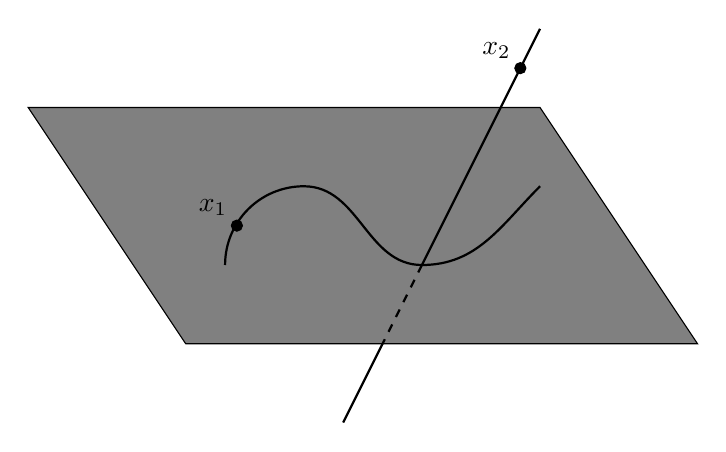
\begin{tikzpicture}
  \draw [fill=gray] (-.5,-1) -- (6,-1) -- (4,2) -- (-2.5,2) -- (-.5,-1);
  \draw [thick] (0,0) to [out=90,in=180] (1,1) to [out=0,in=180] (2.5,0) to [out=0,in=-135] (4,1);
  \draw [thick] (2.5,0) to (4,3);
  \draw [thick,dashed] (2.5,0) to (2,-1);
  \draw [thick] (2,-1) -- (1.5,-2);
  \draw [fill] (3.75,2.5) circle [radius=2pt] node[above left]{$x_2$};
  \draw [fill] (.15,.5) circle [radius=2pt] node[above left]{$x_1$};
 \end{tikzpicture}
\end{center}
 
 The invariants which we need to consider will hence be of the form
 \[
  \langle i^*\eta_i\psi_1^j,\rho^h\rangle_{\Q{0}{2}{Y}{\beta^{(0)}}}\langle \rho_h,\mathbbm 1_{X}\rangle_{\Q{0}{(m^{(1)},0)}{X|Y}{\beta^{(1)}}}, \quad h\in\{1,\ldots,k'\}
 \]
 
 Consider the following dimensional computation:
\begin{align*}
 0\leq \codim \rho^h &= \dim Y-\codim \rho_h \\
 &= \dim Y-\vdim \Q{0}{(m^{(1)},0)}{X|Y}{\beta^{(1)}} \\
 &= \dim Y-(\dim X-3-K_{X}\cdot \beta^{(1)}+2-m^{(1)})\\
 &= K_Y \cdot \beta^{(1)}-Y \cdot \beta^{(1)}+m^{(1)}\leq 0
\end{align*}
 where the last equality follows from adjunction, and the inequality follows from $K_Y\leq 0$ and $m^{(1)}\leq Y \cdot \beta^{(1)}$.
This shows that the only non-trivial contributions are due to the classes $\beta^{(1)}$ such that $K_Y \cdot \beta^{(1)}=0$, and the order of tangency is forced to be maximal, i.e. $m^{(1)}=Y \cdot \beta^{(1)}$. Furthermore, the only relevant insertions are $\rho^1=\mathbbm 1_Y$ and $\rho_1=[pt_Y]$. Finally, $m^{(1)}=Y \cdot \beta^{(1)}$ implies that
\[
 m=\alpha_1=Y \cdot \beta^{(0)}+m^{(1)}=Y \cdot \beta,
\]
hence the boundary contributions do not show up until the very end of the process of ``increasing the multiplicity''.

The remaining term in $T_{(m)}^{X|Y}(z,\beta)$ is $m(\ev_1)_*[\Q{0}{(m,0)}{X|Y}{\beta}]^\text{vir}$; notice that it only gets insertions from the cohomology of $X$ (restricted to $Y$). On the other hand
\[
 \vdim \Q{0}{(m,0)}{X|Y}{\beta}=\dim X-3 -K_X \cdot \beta +2-m \geq r-1
\]
because $m\leq Y\cdot\beta$ and $-(K_X+Y).\beta\geq 0$, by adjunction, projection formula, and for every effective curve class $\beta$ (coming from $Y$, but saying this is superfluous by Lefschetz's hyperplane theorem as we have already remarked); since the restriction of the class $[pt_X]$ to $Y$ vanishes, the only insertion that contributes is $\eta_1$ (by definition of a dual basis, all other dimension 1 classes vanish when restricted to $Y$), forcing the equality $m=Y\cdot\beta$, so that again this correction term is non-trivial only in the last step of the algorithm.

So, in the end, we see that equation \ref{eqn:G} reduces to
\begin{align*}
 &\prod_{j=0}^{Y\cdot\beta}(Y+jz) S_0^X(z,\beta) = T_{(Y\cdot\beta)}^{X|Y}(z,\beta) \\
 &= \sum_{i=1,\ldots,k;j\geq 0}z^{j+1}\eta^i\langle \rho_i\psi_1^j,\mathbbm 1_{Y}\rangle_{\Q{0}{2}{Y}{\beta}} \\
 &+\sum_{\substack{0<\beta^{(0)}<\beta \\ \beta^{(0)}+\beta^{(1)}=\beta}}z^{j+1}\eta^i\langle \rho_i\psi_1^j,\mathbbm 1_{Y}\rangle_{\Q{0}{2}{Y}{\beta^{(0)}}}(Y\cdot\beta^{(1)})\langle [pt_Y],\mathbbm 1_{X}\rangle_{\Q{0}{(Y\cdot\beta^{(1)},0)}{X|Y}{\beta^{(1)}}}\\
 &+\eta^1(Y\cdot\beta)\langle [pt_Y],\mathbbm 1_{X}\rangle_{\Q{0}{(Y\cdot\beta,0)}{X|Y}{\beta}}
\end{align*}
if $\beta$ is such that $K_Y\cdot\beta=0$ (which implies $K_Y\cdot\beta^{(1)}=0$ as well, for every effective decomposition $\beta=\beta^{(0)}+\beta^{(1)}$, due to the semi-positivity assumption on $Y$); while, if $K_Y\cdot\beta<0$, it simply reduces to
\[
 \prod_{j=0}^{Y\cdot\beta}(Y+jz) S_0^X(z,\beta)= \sum_{i=1,\ldots,k;j\geq 0}z^{j+1}\eta^i\langle \rho_i\psi_1^j,\mathbbm 1_{Y}\rangle_{\Q{0}{2}{Y}{\beta}} = i_*S_0^Y(z,\beta).
\]


The proof of the first claim is now evident. We are left with evaluating $P(q)$.

In order to do that, we use again Gathmann's algorithm, this time in the opposite direction, to go all the way back to $X$; so it starts:
\[
 [\Q{0}{(Y \cdot \beta,0)}{X|Y}{\beta}]^\text{vir}=(Y+(Y\cdot\beta-1)\psi_1)[\Q{0}{(Y\cdot\beta-1,0)}{X|Y}{\beta}]^\text{vir}-[D_{Y\cdot\beta}^{\mathcal Q}(X|Y,\beta)]^\text{vir}
\]
When looking at the boundary, the invariants that come into play are of the form
\[
 \langle [pt_Y],\rho^h\rangle_{\Q{0}{2}{Y}{\beta^{(0)}}}\langle \rho_h,\mathbbm 1_{X}\rangle_{\Q{0}{(Y\cdot(\beta-\beta^{(0)})-1,0)}{X|Y}{\beta-\beta^{(0)}}}
\]
but notice that they must vanish by dimensional reasons, since
\[
 \codim(\rho^h)=\dim Y-3+2-K_Y\cdot\beta^{(0)}-\dim Y=-1.
\]
So
\begin{align*}
 & (Y\cdot\beta)\langle [pt_Y],\mathbbm 1_{X}\rangle_{\Q{0}{(Y\cdot\beta,0)}{X|Y}{\beta}} = \\
 & = (Y\cdot\beta)\int_{[\Q{0}{2}{X}{\beta}]^{\text{vir}}}\ev_1^*(\eta_1)\prod_{j=0}^{Y\cdot\beta-1}(\ev_1^*Y+j\psi_1) = \\
 & = (Y\cdot\beta)!\langle[pt_X]\psi_1^{Y\cdot\beta-1},\mathbbm 1_X\rangle_{\Q{0}{2}{X}{\beta}}.
\end{align*}
the second equality because $Y\cdot\eta_1=[pt_X]$ and $Y^2.\eta_1=0$.
\end{proof}

\begin{cor}
 If $Y$ is itself Fano, then there is no correction term
 \[
  \sum_{\beta\geq 0} q^\beta\prod_{j=0}^{Y\cdot\beta}(Y+jz)S_0^X(z,\beta) = i_*S_0^Y(z,q)
 \]
\end{cor}

\begin{cor}
 Let $Y_5$ be the quintic three-fold in $\PP^4$. Then
 \[
  i_*S_0^{Y_5}(z,q)=\frac{I_{\text{small}}^{Y_5}(z,q)}{P^{Y_5}(q)},
 \]
where
\[
 I_{\text{small}}^{Y_5}(z,q)=5H+\sum_{d>0}\frac{\prod_{j=0}^{5d}(H+jz)}{\prod_{j=0}^{d}(H+jz)^5}q^d
\]
and
\[
 P^{Y_5}(q)=1+\sum_{d>0}\frac{(5d)!}{(d!)^5}q^d.
\]
\end{cor}

\begin{remark}
 This formula (and, more generally, formulae for concavex bundles over products of projective spaces) was already obtained in \cite[Theorem 1]{CZ-mirror} via equivariant localisation.
\end{remark}

\subsection{Comparison with the work of Ciocan-Fontanine and Kim}

We would like to compare our formula to \cite[Corollary 5.5.1]{CF-K-wallcrossing}.

In \cite[Section 5]{CF-K-wallcrossing} they introduce (in the more general context of $\epsilon$-stable quasimaps to GIT quotients)
\begin{itemize}
 \item the $J^{\epsilon}$-function:
 \[
  J^\epsilon({\bf t}, z)=\sum_{k\geq 0,\beta\geq 0}q^\beta(\ev_\bullet)_*\left(\frac{\prod_{i=1}^k ev_i^*({\bf t})}{k!}\cap\operatorname{Res}_{F_0}[\QGe{0}{k}{Y}{\beta}]^{\text{vir}}\right)
 \]
\item the $S^\epsilon$-operator
\[
 S^\epsilon(z)(\gamma)=\sum_{m\ge 0,\beta\ge 0}\frac{q^\beta}{m!} 
(ev_1)_*\left(\frac{[\Qe{0}{2+m}{Y}{\beta}]^{\text{vir}}}{z-\psi}ev_2^*(\gamma)\prod_{j=3}^{2+m}ev_j^*({\bf t})\right)
\]
\item the $P^\epsilon$-series
\[
 P^\epsilon({\bf t}, z)=\sum_h\rho^h\sum_{m\geq 0,\beta\geq 0} \frac{q^\beta }{m!}
[\QGe{0}{1+m}{Y}{\beta}]\cap \ev_1^*(\rho_h p_\infty)
\]
where $p_\infty\in H^*_{\Gm}(\PP^1)$ is defined via its restrictions to the $\Gm$-fixed points: $p_{\infty|0}=0,p_{\infty|\infty}=-z$.
\end{itemize}
They prove by localisation that \cite[Theorem 5.4.1]{CF-K-wallcrossing}
\[
 J^\epsilon(z)=S^\epsilon(z)(P^\epsilon).
\]
Furthermore, they prove that, restricting to ${\bf t}=0$ and semi-positive targets, the only class that matches non-trivially with $P^\epsilon_{|{\bf t}=0}$ is $[pt_Y]$, and the above formula takes the simpler form of a product \cite[Corollary 5.5.1]{CF-K-wallcrossing}
\[
 \frac{J^\epsilon |_{{\bf t}=0}}{\langle [pt_Y],  P^\epsilon|_{{\bf t}=0}\rangle}=\mathbbm 1_Y+\sum_h\rho^h(\sum_{\beta\neq 0}q^\beta\langle\frac{\rho_h}{z-\psi},\mathbbm 1_Y\rangle_{0,2,\beta}^\epsilon).
\]
Notice that the restriction of $S^\epsilon(z)(\mathbbm 1_Y)$ to ${\bf t}=0$ that appears on the RHS of this formula coincides with what we have called $S^Y_0(z,q)$ above.

They also observe that, if we write the $\frac{1}{z}$-expansion of $J^{\epsilon}_{{\bf t}=0}$ as
\[
 J^{\epsilon}_{{\bf t}=0}=J^{\epsilon}_{0}(q)\mathbbm 1_Y+O(\frac{1}{z})
\]
then $\langle [pt_Y],  P^\epsilon|_{{\bf t}=0}\rangle=J^{\epsilon}_{0}(q)$.

Let us look more closely at $J^{\epsilon}_{{\bf t}=0}=\sum_{\beta\geq 0}q^\beta(\ev_\bullet)_*\left(\operatorname{Res}_{F_0}[\QGe{0}{0}{Y}{\beta}]^{\text{vir}}\right)$. Recall that in our context $Y\subseteq X$ is a very ample hypersurface and $X$ is toric Fano. Furthermore, set $\epsilon=0^+$. We have the following diagram:

\begin{center}
 \begin{tikzcd}
  \QG{0}{0}{Y}{\beta}\ar[d,hook,"\iota"]\ar[dr,phantom,"\Box"] & F_0^Y\ar[d]\ar[l,hook]\ar[r,"\ev_{\bullet}"] & Y\ar[d,hook,"i"] \\
  \QG{0}{0}{X}{\beta} & F_0^X\ar[l,hook]\ar[r,"\ev_{\bullet}"] & X
 \end{tikzcd}
\end{center}

\begin{itemize}[leftmargin=*]
 \item By a slight generalisation of \cite[Propositions 6.2.2 and 6.2.3]{CFKM}, $\iota_*[\QG{0}{0}{Y}{\beta}]^{\text{vir}}=e(\pi_* E^Y_{0,0,\beta}(z))\cap[\QG{0}{0}{X}{\beta}]^{\text{vir}}$ as $\Gm$-equivariant classes, where $\pi$ is the universal curve on $\QG{0}{0}{X}{\beta}$ and $E^Y_{0,0,\beta}(z)$ is the equivariant line bundle on it associated to $\mathcal O_X(Y)$. This is analagous to the bundle $L_Y$ used in the definition of relative quasimaps (see \S \ref{Subsection relative stable quasimaps}).
\item Since the fibers of $\pi$ are irreducible (by the stability condition and the fact that there are no markings, there can only be the parametrised component), the following splitting holds:
 \[
  e(\pi_* E^Y_{0,0,\beta}(z))=\prod_{j=0}^{Y\cdot\beta} c_1(\sigma_0^* E^Y_{0,0,\beta}(z)\otimes \omega_{\pi}^{\otimes j})
 \]
coming from evaluating at (the $j$-th order infinitesimal thickening of) the zero section $\sigma_0$ and the jet bundles exact sequence:
\begin{center}
 \begin{tikzcd}
  0\ar[r] & \pi_* (E^Y_{0,0,\beta}(-j\sigma_0))\ar[r] & \pi_* E^Y_{0,0,\beta}\ar[r] & \sigma_0^*\operatorname{P}^{j-1}(E^Y_{0,0,\beta}) \ar[r] & 0 \\
  0\ar[r] & \Omega_\pi^{\otimes j}\otimes E^Y_{0,0,\beta}\ar[r] & \operatorname{P}^{j}(E^Y_{0,0,\beta}) \ar[r] & \operatorname{P}^{j-1}(E^Y_{0,0,\beta}) \ar[r] & 0
 \end{tikzcd}
\end{center}
which, restricting to $F_0^X$, gives:
\[
 \iota_*[F_0^Y]^{\text{vir}}=\prod_{j=0}^{Y\cdot\beta}(Y+iz)[F_0^X]^{\text{vir}}.
\]
 \item The small $J^{0^+}$-function for toric varieties has been evaluated by Givental \cite{Givental-equivariantGW}\cite[Definition 7.2.8]{CF-K}:
 \[
  (\ev_{\bullet})_*\frac{[F_0^X]^{\text{vir}}}{e(N_{F_0/\QG{0}{0}{X}{\beta}})}=\prod_{\rho\in\Sigma_X(1)}\frac{\prod_{j=-\infty}^0(D_{\rho}+jz)}{\prod_{j=-\infty}^{\int_{\beta}D_{\rho}}(D_\rho+jz)}=\frac{\prod_{\substack{\rho\in\Sigma_X(1)\colon D_\rho.\beta\leq 0 \\ j=\int_{\beta}D_\rho,\ldots,0}}(D_{\rho}+jz)}{\prod_{\substack{\rho\in\Sigma_X(1)\colon D_\rho.\beta> 0 \\ j=1,\ldots,\int_{\beta}D_\rho}}(D_{\rho}+jz)}
 \]
So, using $\sum_{\rho\in\Sigma_X(1)} D_{\rho}=-K_X$ and $(Y+K_X).\beta=0$, we see that
\[
 J^Y_0(q)=\sum_{\beta\geq 0}q^\beta(Y\cdot\beta)!\frac{\prod_{\rho\in\Sigma_X(1)\colon D_\rho.\beta< 0}(-1)^{-D_{\rho}.\beta}(-D_{\rho}.\beta)!}{\prod_{\rho\in\Sigma_X(1)\colon D_\rho.\beta> 0}(D_{\rho}.\beta)!}
\]
\item Since $X$ is Fano, $J^X_{|{\bf t}=0}=S^X_{|{\bf t}=0}(\mathbbm 1_X)$.
\item The coefficient $\langle[pt_X]\psi_1^{Y\cdot\beta-1},\mathbbm 1_X\rangle_{\Q{0}{2}{X}{\beta}}$ that appears in our $P$-series (multiplied by $(Y\cdot\beta)!$), can be deduced from the expansion of $S^X_{|{\bf t}=0}(\mathbbm 1_X)$ given above, and it turns out to be
\[
 \langle [pt_X],S^X_{|{\bf t}=0}(\mathbbm 1_X)\rangle[z^{Y\cdot\beta}]=\frac{\prod_{\rho\in\Sigma_X(1)\colon D_\rho.\beta< 0}(-1)^{-D_{\rho}.\beta}(-D_{\rho}.\beta)!}{\prod_{\rho\in\Sigma_X(1)\colon D_\rho.\beta> 0}(D_{\rho}.\beta)!}.
\]

\end{itemize}

So we may conclude that the $i_*$ of \cite[Corollary 5.5.1]{CF-K-wallcrossing} coincides with our Equation \ref{eqn:mirror}.

\appendix

\section{The Comparison Morphism}

We summarise the existence of the comparison morphism for $\PP^r$ and how it implies that GW and quasimap invariants of projective space coincide. This has been proven in \cite[Theorem 3]{MOP} and \cite[Section 4.3]{Manolache-Push} (but see also \cite[Proposition 4.1]{Bertram} and \cite[Theorem 7.1]{Popa-Roth} for inspiration). We shall try to clarify as many details as possible, for our own benefit and, hopefully, that of the novice reader.

In order to give a morphism $\comp\colon\M{g}{n}{\PP^r}{d}\to\Q{g}{n}{\PP^r}{d}$ we need to be able to canonically associate a family of quasimaps on a base $S$ to any family of stable maps on the same base.

The pointwise construction is the following: a stable map has no base points, so the only thing that might prevent it from being a stable quasimap is the presence of rational tails (of positive degree, by the stable maps stability condition). Let $C=C^{(0)}\sqcup_{q_i}R_i$ be the source curve; the rational tail $R_i$ has degree $d_i$ and is joined to the permanent curve $C^{(0)}$ at the node $q_i$, which is the only special point on $R_i$; hence all the markings belong to $C^{(0)}$. The map to $\PP^r$ is equivalent to the data of a line bundle $L=f^*\mathcal O_{\PP^r}(1)$ on $C$ and $r+1$ sections $s_0,\ldots,s_r$ thereof. We associate to such a stable map the quasimap $(C^{(0)},\mathbf x; L_{|C^{(0)}}\otimes\mathcal O_{C^{(0)}}(\sum_{i}d_iq_i);\hat s_0,\ldots,\hat s_r)$, where $\hat s_j$ is the restriction of $s_j$ to $C^{(0)}$, seen as a section of $L_{|C^{(0)}}\otimes\mathcal O_{|C^{(0)}}(\sum_{i}d_iq_i)$ through the inclusion $L_{|C^{(0)}}\hookrightarrow L_{|C^{(0)}}\otimes\mathcal O_{C^{(0)}}(\sum_{i}d_iq_i)$. Notice that the resulting quasimap has a base-point of order $d_i$ at $q_i$.

The construction in families requires us to find a line bundle on the universal curve that is trivial on the rational tails and relatively ample elsewhere. This can be performed at the level of Picard stacks: let $\mathfrak{Pic}_{g,n}^{d,\text{st}}$ be the open substack of $\mathfrak{Pic}(\pi\colon\mathfrak{C}_{g,n}\to\mathfrak{M}_{g,n})$ obtained by requiring that the total degree of the line bundle is $d$, the multi-degree is nonnegative and $\mathcal L\otimes\omega_{\pi}^{\text{log}}$ is ample relative to $\pi$, where $\mathcal L$ is the universal line bundle. Let $T^{\delta}$ be the locus in the universal curve over $\mathfrak{Pic}_{g,n}^{d,\text{st}}$ spanned by rational tails on which $\mathcal L$ has degree $\delta$; this is a Cartier divisor by deformation theory and smoothness of the stack $\mathfrak{C}_{\mathfrak{Pic}}$. Notice that $T^{\delta_0}$ and $T^{\delta_1}$ (say $\delta_0<\delta_1$) do intersect in a stratum of codimension 1 in both of them, where the rational tail splits into two rational components, the furthest from $C^{(0)}$ having degree $\delta_0$.

[FIGURE]

\emph{Claim:} the line bundle $\mathcal M=\mathcal L\otimes\omega_{\pi}^{\text{log}}\otimes\bigotimes_{0<\delta\leq d}\mathcal O_{\mathfrak C}((\delta-1) T^\delta)$ on $\mathfrak{C}_{\mathfrak{Pic}}$ has degree 0 on every component of every rational tail, and is $\pi$-relatively ample elsewhere.

\begin{proof}

Consider a curve $C^{(0)}\sqcup_q R$ with a rational tail of degree $\delta$, such that $R$ consists of $n$ many components $R^{(1)
},\ldots,R^{(n)}$, each of degree $\delta^{(1)},\ldots,\delta^{(n)}$ respectively, numbered from the closest to the farthest from $C^{(0)}$; set $T_i=\bigcup_{j=i}^n R_j$ and $\epsilon_i=\delta-1-\sum_{j=1}^{i-1}\delta_j$.

[FIGURE]

A general one-parameter family in $\mathfrak{Pic}_{g,n}^{d,\text{st}}$ will give us a smoothing of such a curve; the universal curve over such a family is a normal surface $S$; we can compute the degree of the restriction of $\mathcal M$ to components of the central fiber of this family by first restricting $\mathcal M$ to $S$, and then using intersection theory on this normal surface.

Notice that restricting $\bigotimes_{0<\delta\leq d}\mathcal O_{\mathfrak C}((\delta-1) T^\delta)$ to this family gives $\mathcal O_S(\sum_{j=1}^n\epsilon_jT_j)$. Since $R^{(i)}$ is a $(-2)$-curve for $i=1,\ldots,n-1$, and $R^{(n)}$ is a $(-1)$-curve, we get

\[
  R^{(i)}.T_j =
  \begin{cases}
    0, & \text{for } j<i \\
    -1, & \text{for } j=i \\
    1, & \text{for } j=i+1 \\
    0 & \text{for } j>i+1 \\
  \end{cases}
\]
hence $\deg(\mathcal M_{|R^{(i)}})=\delta^{(i)}-\epsilon_i+\epsilon_{i+1}=0$ for $i=1\ldots,n-1$, while for $i=n$ it is $\delta^{(n)}-1-\epsilon_n=0$, as $\omega^{\text{log}}$ is trivial on the $(-2)$ curves and has degree $-1$ on $R^{(n)}$. The last assertion of the claim follows from the stability condition and the fact that $O_{\mathfrak C}(T^\delta)$ is effective when restricted to $C^{(0)}$.
\end{proof}

By taking the relative Proj construction we obtain another curve $\hat{\mathfrak C}=\underline\Proj_{\mathfrak{Pic}}\left(\bigoplus_{k\geq 0}\pi_*\mathcal M^{\otimes k}\right)$ over $\mathfrak{Pic}_{g,n}^{d,\text{st}}$, with a map $\rho$ that contracts the rational tails
\bcd
\mathfrak C_{\mathfrak{Pic}}\ar[r,"\rho"]\ar[dr,"\pi"] & \hat{\mathfrak C} \ar[d,"\pi'"]\\
 & \mathfrak{Pic}_{g,n}^{d,\text{st}}
\ecd
It is flat because it is a family of genus $g$ curves over a reduced base. Furthermore, it can be checked by cohomology and base-change \cite[Theorem 12.11]{HAR}\cite[Corollary 1.5]{Knudsen} (notice that the fibers of $\rho$ are either points or rational curves) that $\hat{\mathcal L}=\rho_*\left(\mathcal L\otimes \bigotimes_{0<\delta\leq d}\mathcal O_{\mathfrak C}(\delta T^\delta)\right)$ is a line bundle on $\hat{\mathfrak C}$ of degree $d$ relative to $\pi'$ (such that $\rho^*\hat{\mathcal L}\simeq\mathcal L\otimes \bigotimes_{0<\delta\leq d}\mathcal O_{\mathfrak C}(\delta T^\delta)$), hence the universal property gives us a commutative diagram (with Cartesian square)
\bcd
\mathfrak C_{\mathfrak{Pic}}\ar[r,"\rho"]\ar[dr,"\pi"] & \hat{\mathfrak C} \ar[d,"\pi'"]\ar[dr,phantom,"\square"]\ar[r] & \mathfrak C_{\mathfrak{Pic}}\ar[d,"\pi"] \\
 & \mathfrak{Pic}_{g,n}^{d,\text{st}}\ar[r,"\comp '"] & \mathfrak{Pic}_{g,n}^{d,\text{st}}
\ecd
The very same construction, with the line bundles pulled back from the Picard stack, and the sections of $\mathcal L$ seen as sections of $\mathcal L\otimes \bigotimes_{0<\delta\leq d}\mathcal O_{\mathfrak C}(\delta T^\delta)$ through the inclusion of line bundles ($\mathcal O_{\mathfrak C}(T^\delta)$ is effective), and descended to sections of $\hat{\mathcal L}$ on $\hat{\mathfrak C}$ gives us the comparison morphism $\comp\colon \M{g}{n}{\PP^r}{d}\to\Q{g}{n}{\PP^r}{d}$, fitting in a commutative diagram
\bcd
\M{g}{n}{\PP^r}{d} \ar[d,"\nu_{\mathcal M}"]\ar[r,"\comp"] & \Q{g}{n}{\PP^r}{d}\ar[d,"\nu_{\mathcal Q}"] \\
\mathfrak{Pic}_{g,n}^{d,\text{st}}\ar[r,"\comp '"] & \mathfrak{Pic}_{g,n}^{d,\text{st}}
\ecd
and, as before,
\bcd
\mathcal C_{\mathcal M}\ar[r,"\rho"]\ar[dr,"\pi_{\mathcal M}"] & \hat{\mathcal C}=\comp^*\mathcal C_{\mathcal Q} \ar[d,"\hat\pi"]\ar[dr,phantom,"\square"]\ar[r] & \mathcal C_{\mathcal Q}\ar[d,"\pi_{\mathcal Q}"] \\
 & \M{g}{n}{\PP^r}{d}\ar[r,"\comp"] & \Q{g}{n}{\PP^r}{d}
\ecd

The comparison between virtual fundamental classes is best outlined in the arXiv version of \cite[Remark 5.20]{Manolache-Push}. Call $\nu_{\mathcal M}'=\comp'\circ\nu_{\mathcal M}$. We may endow it with an obstruction theory by means of
\bcd
\nu_\mathcal M^*\mathbb L_{\comp'}\ar[d]\ar[r] & \mathbb E_{\nu'_\mathcal M} \ar[d]\ar[r] & \mathbb E_{\nu_\mathcal M} \ar[d]\ar[r,"{[1]}"] & {}\\
\nu_\mathcal M^*\mathbb L_{\comp'}\ar[r] & \mathbb L_{\nu'_\mathcal M} \ar[r] & \mathbb L_{\nu_\mathcal M} \ar[r,"{[1]}"] & {}
\ecd

Notice that $\comp'$ is a morphism (not of DM type) between smooth Artin stacks, hence we can only deduce that $\mathbb L_{\comp'}$ is supported in $[-1,1]$. It is therefore easily seen that $\mathbb E_{\nu'_\mathcal M}$ is also supported in $[-1,1]$; in order to show that it is actually a perfect obstruction theory, consider the long exact sequence
\begin{align*}
 0 &\to h^{-1}\nu_\mathcal M^*\mathbb L_{\comp'}\to h^{-1}\mathbb E_{\nu'_\mathcal M} \to h^{-1}\mathbb E_{\nu_\mathcal M} \\
 &\to h^{0}\nu_\mathcal M^*\mathbb L_{\comp'}\to h^{0}\mathbb E_{\nu'_\mathcal M} \to h^{0}\mathbb E_{\nu_\mathcal M} \\
 &\to h^{1}\nu_\mathcal M^*\mathbb L_{\comp'}\to h^{1}\mathbb E_{\nu'_\mathcal M} \to 0
\end{align*}
and observe that, dually, $h^{-1}\nu_\mathcal M^*\mathbb T_{\comp'}$ injects into $h^{0}\mathbb E^\vee_{\nu_\mathcal M}\simeq h^{0}\mathbb T_{\nu_\mathcal M}$, because every infinitesimal automorphism of the rational tail induces a nontrivial deformation of the stable map (since the degree of the latter is positive on every component of the rational tail); we conclude that $h^{1}\mathbb E_{\nu'_\mathcal M}=0$.

\emph{Claim:} there is a morphism of obstruction theories $\comp^*\mathbb E_{\nu_\mathcal Q}\to\mathbb E_{\nu_\mathcal M}$ \cite[Lemma 4.19]{Manolache-Push}.

Dually, $\mathbb E^\vee_{\nu_\mathcal M}=R^\bullet\pi_{\mathcal{M}*}\mathcal L^{\oplus r+1}=R^\bullet\hat\pi_*(\rho_*\mathcal L^{\oplus r+1})$, while, by cohomology and base-change, $\comp^*\mathbb E^\vee_{\nu_\mathcal Q}=R^\bullet\hat\pi_*(\hat{\mathcal L}^{\oplus r+1})$, where $\hat{\mathcal L}=\rho_*\left(\mathcal L\otimes \bigotimes_{0<\delta\leq d}\mathcal O_{\mathfrak C}(\delta T^\delta)\right)$, so $\mathbb E^\vee_{\nu_\mathcal M}\to\comp^*\mathbb E^\vee_{\nu_\mathcal Q}$ comes from the inclusion of line bundles on $\mathcal C_\mathcal M$
\[
\mathcal L\hookrightarrow \mathcal L\otimes \bigotimes_{0<\delta\leq d}\mathcal O_{\mathfrak C}(\delta T^\delta).
\]

\emph{Claim:} this morphism factors through $\mathbb E_{\nu'_\mathcal M}$.

\bcd
& \comp^*\mathbb E_{\nu_\mathcal Q}\ar[dl,dashed,"\exists ?"]\ar[d]\ar[dr,"\phi"] & \\
\mathbb E_{\nu'_\mathcal M} \ar[r] & \mathbb E_{\nu_\mathcal M}\ar[r] & \nu_\mathcal M^*\mathbb L_{\comp'}[1]
\ecd

In order to prove that the dashed arrow exists, we need to show that $\phi$ is the zero map. Dually, we look at $\nu_\mathcal M^*\mathbb T_{\comp'}[-1]\xrightarrow{\phi^\vee} R^\bullet\hat\pi_*(\hat{\mathcal L}^{\oplus r+1})$. Notation: call $R$ the rational tail, joined at the rest of the curve (which we denote by $(C^{(0)},\mathbf p)$ as a marked curve), at the node $q$, which we may occasionally think of as a (smooth) point on $C^{(0)}$. We claim that:
\begin{itemize}
 \item $h^0(\phi^\vee)$ is zero because: the LHS involves automorphisms of the rational tail that leave $C^{(0)}$ fixed, while the RHS involves deformations of $C^{(0)}$, so there is no possible interference.
 \item $h^1(\phi^\vee)$ is zero because: \textcolor{red}{this is slightly awkward.} There are two types of possible contributions to the LHS. They correspond to either moving the node $q$ along $C^{(0)}$, or smoothing it. The former appears in the relative tangent of $\chi'$ only if the marked curve $(C^{(0)},\mathbf p)$ has no automorphisms that may ``move $q$ back'', i.e. $(C^{(0)},\mathbf p)$ is a stable pointed curve. The latter matters only if $(C^{(0)},q,\mathbf p)$ has no moduli, i.e. $(C^{(0)},\mathbf p)$ is a rational tail with less than 3 markings. \textcolor{red}{I will try to justify why the first type vanishes under $h^1(\phi^\vee)$, and leave the second type because I do not understand it as yet.} Look at the long exact sequence
 
\begin{align*}
  0 &\to \Hom(\Omega_{C^{(0)}},\mathcal O_{C^{(0)}}(-q-\sum p_i)) &\to \Hom(\Omega_{C^{(0)}},\mathcal O_{C^{(0)}}(-\sum p_i)) &\to \\
  T_{C^{(0)},q} &\to \Ext^1(\Omega_{C^{(0)}},\mathcal O_{C^{(0)}}(-q-\sum p_i)) &\to \Ext^1(\Omega_{C^{(0)}},\mathcal O_{C^{(0)}}(-\sum p_i)) &\to 0
 \end{align*}
We are interested in what happens to
\[
 \frac{T_{C^{(0)},q}}{\operatorname{Im}\left( \Hom(\Omega_{C^{(0)}},\mathcal O_{C^{(0)}}(-\sum p_i)) \right)}
\]
under $h^1(\phi^\vee)$. If we can show that $h^1(\phi^\vee)$ factors through $\Ext^1(\Omega_{C^{(0)}},\mathcal O_{C^{(0)}}(-\sum p_i))$ we are in business. Indeed the natural maps
\bcd
\Def_L\ar[d]\ar[r] & \Def_{(C,L)}\ar[d]\ar[r] & \Def_C\ar[d] \\
H^1(\mathcal O_C)\ar[r] & H^1(L^{\oplus r+1})\ar[r] & H^1(f^*T_{\PP^r})
\ecd
show that $h^1(\phi^\vee)$ factors through
\[
\Ext^1(\Omega_{C^{(0)}},\mathcal O_{C^{(0)}}(-q-\sum p_i))\to \Ext^1(\Omega_{C^{(0)}},\mathcal O_{C^{(0)}})\to \Ext^1(f^*\Omega_{\PP^r},\mathcal O_{C^{(0)}})\simeq H^1(f^*T_{\PP^r}).
\]
 \item $h^2(\phi^\vee)$ is zero because: $\mathbb E^\vee_{\nu'_\mathcal M}$ is supported in $[0,1]$.
\end{itemize}
Now the cone $C(\phi)$ gives an obstruction theory relative to $\comp$. A priori, it is supported in $[-2,0]$. By the octahedral axiom
\begin{center}
 \begin{tikzcd}[cramped]
  \comp^*\mathbb E_{\nu_\mathcal{Q}} \ar[dd,"\phi"]\ar[rrdd,"\phi'"] & & & & & & \\
& & & & & & \\
\mathbb E_{\nu'_\mathcal{M}}\ar[dd]\ar[rr] & & \mathbb E_{\nu_\mathcal{M}} \ar[rrrr]\ar[dr] & & & & \nu_{\mathcal M}^*\mathbb L_{\comp'}{[1]} \\
& & & C(\phi')\ar[urrr] & & & \\
C(\phi) \ar[urrr] & & & & & & 
 \end{tikzcd}
\end{center}
it is enough to observe that $C(\phi')$ is supported in $[-1,0]$ \cite[Lemma 4.20]{Manolache-Push} and that $\nu_{\mathcal M}^*\mathbb L_{\comp'}{[1]}$ is supported in degrees $[-2,0]$, in order to conclude that $C(\phi)=\mathbb E_{\comp}$ is a perfect obstruction theory. The conclusion that
\[
 \comp_*[\M{g}{n}{\PP^r}{d}]^{\text{vir}}=[\Q{g}{n}{\PP^r}{d}]^{\text{vir}}
\]
follows from the connectedness of $\M{g}{n}{\PP^r}{d}$ \cite{KP} (hence of $\Q{g}{n}{\PP^r}{d}$) and an application of the virtual push-forward theorem \cite[Proposition 4.21]{Manolache-Push}.

We shall now explain with an example the reason why a naive attempt to extend the comparison morphism to a general toric variety fails. The problem in a nutshell is that not all toric divisors are nef: a rational tail contained in a divisor which is not nef may have negative degree $-d$ with respect to the corresponding line bundle; when contracting such a rational tail, we shall take the line bundle $L(-dq)$, but what to do with the sections? We would like to divide them by $z^d$, where $z$ is a local coordinate around $q$, but no condition forces such a divisibility to happen. Otherwise said, there is now an inclusion $L_{|C^{(0)}}(-dq)\hookrightarrow L_{|C^{(0)}}$, but the (restriction of the) given sections of $L$ do not necessarily live in the image of $H^0(C^{(0)},L_{|C^{(0)}}(-dq))\hookrightarrow H^0(C^{(0)},L_{|C^{(0)}})$.

A concrete example is found when looking at the Hirzebruch surface $\mathbb F_1=\operatorname{Bl}_{p}\PP^1$.
\begin{figure}
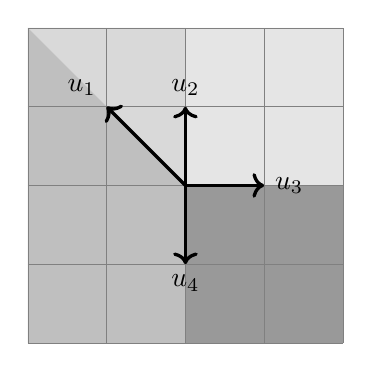
\begin{tikzpicture}
\path [fill=black!10!white] (0,0) -- (2,0) -- (2,2) -- (0,2) -- (0,0);
\path [fill=black!15!white] (0,0) -- (-2,2) -- (0,2) -- (0,0);
\path [fill=black!25!white] (0,0) -- (-2,2) -- (-2,-2) -- (0,-2) -- (0,0);
\path [fill=black!40!white] (0,0) -- (0,-2) -- (2,-2) -- (2,0) -- (0,0);
\draw [help lines] (-2,-2) grid (2,2);
\draw [->,very thick] (0,0) -- (-1,1) node[above left]{$u_1$};
\draw [->,very thick] (0,0) -- (0,1) node[above]{$u_2$};
\draw [->,very thick] (0,0) -- (1,0) node[right]{$u_3$};
\draw [->,very thick] (0,0) -- (0,-1) node[below]{$u_4$};
\end{tikzpicture}
\caption{Toric fan for $\mathbb F_1$.}
\end{figure}

\begin{figure}
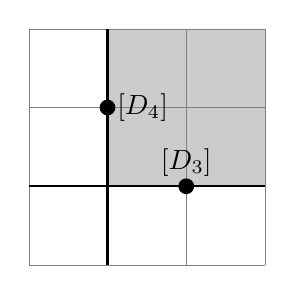
\begin{tikzpicture}
\path [fill=black!20!white] (0,0) -- (2,0) -- (2,2) -- (0,2) -- (0,0);
\draw [help lines] (-1,-1) grid (2,2);
\fill [black] (0,1) circle[radius=.1] node[right]{${[D_4]}$};
\fill [black] (1,0) circle[radius=.1] node[above]{${[D_3]}$};
\draw [thick] (-1,0) -- (2,0);
\draw [thick] (0,-1) -- (0,2);
\end{tikzpicture}
\caption{Nef cone $\operatorname{Nef}(\mathbb F_1)$.}
\end{figure}

\begin{figure}
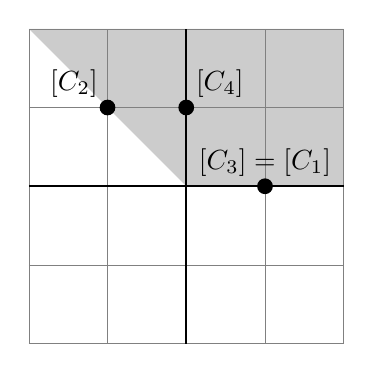
\begin{tikzpicture}
\path [fill=black!20!white] (0,0) -- (2,0) -- (2,2) -- (-2,2) -- (0,0);
\draw [help lines] (-2,-2) grid (2,2);
\fill [black] (0,1) circle[radius=.1] node[above right]{${[C_4]}$};
\fill [black] (1,0) circle[radius=.1] node[above]{${[C_3]}={[C_1]}$};
\fill [black] (-1,1) circle[radius=.1] node[above left]{${[C_2]}$};
\draw [thick] (-2,0) -- (2,0);
\draw [thick] (0,-2) -- (0,2);
\end{tikzpicture}
\caption{Mori cone $\overline{\operatorname{NE}}(\mathbb F_1)$.}
\end{figure}

$\Pic(\mathbb F_1)$ is generated by $[D_3]$ and $[D_4]$, with relations $[D_1]=[D_3]$ and $[D_2]=[D_4]-[D_3]$, and the intersection table is given by
\[
{}
\begin{cases}
 D_3^2=0 \\
 D_3.D_4=0 \\
 D_4^2=1
\end{cases} 
\]
When thinking of $\mathbb F_1$ as a $\PP^1$-bundle over $\PP^1$, $C_1$ and $C_3$ represent the fibers of the bundle (over the toric points of $\PP^1$), while $C_4$ (resp. $C_2$) is the zero/positive (resp. infinity/negative) section; when thinking of $\mathbb F_1$ as $\operatorname{Bl}_{p}\PP^1$, $C_2$ is the exceptional divisor, $C_4$ is the toric line not passing through $p$, and $C_1,C_3$ are the strict transforms of the toric lines through $p$.

Let us look at $\M{0}{2}{\mathbb F_1}{[C_4]}$. Since $[C_4]=[C_2]+[C_3]$, there are going to be maps of the following sort: the source curve is reducible $R_1\sqcup_q R_2$, $R_1$ is mapped isomorphically to a fiber (i.e. in class $[C_3]$) and $R_2$ is mapped isomorphically to $C_2$, all the markings belong to $R_1$. So $R_2$ is a rational tail and deserves to be contracted. Notice that the line bundle $\mathcal O(D_2)$ has degree $-1$ on $R_2$ (and $1$ on $R_1$). In this case everything works well because the corresponding section $u_{2|R_1}$ must vanish at the node, so we can divide it by a chosen (once for all toric line bundles) section of $\mathcal O_{R_1}(q)$.

Consider now $\M{0}{2}{\mathbb F_1}{2[C_2]+[C_3]}$. Certainly there are going to be maps similar to the ones described above, with $R_2$ now covering $C_2$ $2\colon 1$. The point is that $\mathcal O(D_2)$ has degree $-2$ on $R_2$, but $u_{2|R_1}$ doesn't have to vanish at the node of order $2$, so we are in trouble. \textcolor{blue}{Something is going on here: in this case there is a boundary component where the map is of the type that we have just described, and the requirement that $u_{2|R_1}$ vanishes of order $2$ at the node defines precisely the intersection with the main component. Check this. Could we possibly exploit this phenomenon to define a smaller compactification, possibly even smaller than quasimaps?}

\section{Notes on quasimaps}\label{Section quasimap theory}
\subsection{Functoriality and relative obstruction theories} \label{Functoriality of Quasimap Spaces Section}

In the case of stable maps, a morphism $f : X \to Y$ induces a morphism between the corresponding moduli spaces
\begin{equation*}\M{g}{n}{X}{\beta} \rightarrow \M{g}{n}{Y}{f_* \beta} \end{equation*}
given by composition with $f$ (in general this induced morphism may involve stabilisation of the source curve). Because of this, the construction of the moduli space of stable maps is said to be \ildef{functorial}.

It is natural to ask whether the same holds for the moduli space of quasimaps. Since here the objects of the moduli space are not maps, we cannot simply compose with $f$, and indeed it is not immediately clear how we should proceed. In \cite[Section 3.1]{CF-K-wallcrossing} a definition is given when $f$ is an embedding into a projective space; however, this uses the more general language of GIT quotients which we seek to avoid here. As such, we will provide an alternative (but entirely equivalent) construction in the setting of toric varieties, which also relaxes the conditions on the map $f$ and the target $Y$.

\footnote{We should probably look a bit harder to see if the definition exists elsewhere.}

Our approach uses the language of $\Sigma$--collections introduced by D. Cox. This approach is natural insofar as a quasimap is a generalisation of a $\Sigma$--collection. We will refer extensively to \cite{CoxRing} and \cite{CoxFunctor}, which we recommend as an  introduction for any readers unfamiliar with the theory.

Let $X$ and $Y$ be smooth and proper toric varieties with fans $\Sigma_X \subseteq N_X$ and $\Sigma_Y \subseteq N_Y$. Suppose we are given $f : Y \to X$ (which we do not assume to be a toric morphism). By \cite[Theorem 1.1]{CoxFunctor} the data of such a map is equivalent to a $\Sigma_X$--collection on $Y$:
\begin{equation*} ( (L_\rho, u_\rho)_{\rho \in \Sigma_X(1)}, (\varphi_{m_x})_{m_x \in M_X} ) \end{equation*}
In addition, \cite{CoxRing} allows us to describe line bundles on $Y$ and their global sections in terms of the homogeneous coordinates $(z_\tau)_{\tau \in \Sigma_Y(1)}$. All of these observations are combined into the following theorem, which is so useful that we will state it here in its entirety:

\begin{thm} \cite[Theorem 3.2]{CoxFunctor} \label{CoxTheorem} The data of a morphism $f:Y \to X$ is the same as the data of homogeneous polynomials
\begin{equation*} P_\rho \in S^Y_{\beta_\rho} \end{equation*}
for $\rho \in \Sigma_X(1)$, where $\beta_\rho \in \Pic Y$ and $S^Y_{\beta_\rho}$ is the corresponding graded piece of the Cox ring
\begin{equation*}S^Y = k[z_\tau : \tau \in \Sigma_Y(1)]\end{equation*}
This data is required to satisfy the following two conditions:
\begin{enumerate}
\item $\sum_{\rho \in \Sigma_X(1)} \beta_\rho \otimes n_\rho = 0$ in $\Pic Y \otimes N_X$.
\item $(P_\rho(z_\tau)) \notin Z(\Sigma_X) \subseteq \Aaff_k^{\Sigma_X(1)}$ whenever $(z_\tau) \notin Z(\Sigma_Y) \subseteq \Aaff_k^{\Sigma_Y(1)}$.
\end{enumerate}
Furthermore, two such sets of data $(P_\rho)$ and $(P^\prime_\rho)$ correspond to the same morphism if and only if there exists a $\lambda \in \Hom_\Z(\Pic X, \Gm)$ such that
\begin{equation*} \lambda(D_\rho) \cdot P_\rho = P^\prime_\rho \end{equation*}
for all $\rho \in \Sigma_X(1)$. Finally, if we define $\tilde{f}(z_\tau) = (P_\rho(z_\tau))$ then this defines a lift of $f$ to the prequotients:
\bcd
\Aaff_k^{\Sigma_Y(1)} \setminus Z(\Sigma_Y) \ar[r, "\tilde{f}"] \ar[d, "\pi"] & \Aaff_k^{\Sigma_X(1)} \setminus Z(\Sigma_X) \ar[d,"\pi"] \\
Y \ar[r, "f"] & X
\ecd
\end{thm}
\begin{aside} Throughout this section we will stick to the notation established above; in particular we will use $\rho$ to denote a ray in $\Sigma_X(1)$ and $\tau$ to denote a ray in $\Sigma_Y(1)$. \end{aside}

Recall our goal: given a map $f : Y \to X$ we wish to define a ``push-forward'' map:
\begin{equation*} f_* : \Q{g}{n}{Y}{\beta} \to \Q{g}{n}{X}{f_*\beta} \end{equation*}
Consider therefore a quasimap $(C, (L_\tau, u_\tau)_{\tau \in \Sigma_Y(1)}, (\varphi_{m_Y})_{m_Y \in M_Y})$ with target $Y$. Pick data $(P_\rho)_{\rho \in \Sigma_X(1)}$ corresponding to the map $f$, as in the theorem above; we will later see that our construction does not depend on this choice.

The idea of the construction is as follows. Let us pretend for a moment that $C$ is toric and that the quasimap is without basepoints, so that we have an actual morphism $C \to Y$. Then we can lift this morphism to the prequotient as in the following diagram

\bcd
\Aaff_k^{\Sigma_C(1)} \setminus Z(\Sigma_C) \ar[r, "(u_\tau)"] \ar[d] & \Aaff_k^{\Sigma_Y(1)} \setminus Z(\Sigma_Y) \ar[r, "(P_\rho)"] \ar[d] & \Aaff_k^{\Sigma_X(1)} \setminus Z(\Sigma_X) \ar[d] \\
C \ar[r] & Y \ar[r] & X
\ecd
from which it follows that the composition $C \to Y \to X$ is given in homogeneous coordinates by:
\begin{equation*} (P_\rho((u_\tau)_{\tau \in \Sigma_Y(1)}))_{\rho \in \Sigma_X(1)} \end{equation*}
In general of course $C$ is not a toric variety and the quasimap is not basepoint-free. Nevertheless, as we will see, we can still make sense of the expression $P_\rho(u_\tau)$ as a section of a line bundle on $C$. This will allow us to define the pushforward of our quasimap.

Let us begin. For each $\rho$, $P_\rho$ is a polynomial in the $z_\tau$; we can write it as
\begin{equation} \label{Prho} P_\rho(z_\tau) = \sum_{\underline{a}} P_\rho^{\underline{a}}(z_\tau) = \sum_{\underline{a}} \mu_{\underline{a}} \prod_{\tau} z_{\tau}^{a_{\tau}} \end{equation}
where the sum is over a finite number of multindices $\underline{a} = (a_\tau) \in \N^{\Sigma_Y(1)}$ and the $\mu_{\underline{a}}$ are nonzero scalars. For each $\underline{a}$ consider the following line bundle on $C$:
\begin{equation*} \tilde{L}_\rho^{\underline{a}} = \bigotimes_\tau L_\tau^{\otimes a_\tau} \end{equation*}
Then we may take the following section of $\tilde{L}_\rho^{\underline{a}}$:
\begin{equation*} \tilde{u}_\rho^{\underline{a}} = P_\rho^{\underline{a}}(u_\tau) = \mu_{\underline{a}} \prod_\tau u_\tau^{a_\tau} \end{equation*}
Thus each of the terms $P_\rho^{\underline{a}}$ of $P_\rho$ defines a section $\tilde{u}_\rho^{\underline{a}}$ of a line bundle $\tilde{L}_\rho^{\underline{a}}$. But what we want is a single section $\tilde{u}_\rho$ of a single line bundle $\tilde{L}_\rho$. This is where the isomorphisms $\varphi_{m_Y}$ come in.

Recall that we have a short exact sequence:
\begin{equation} \label{Pic short exact sequence for Y} 0 \longrightarrow M_Y \overset{\theta}{\longrightarrow} \Z^{\Sigma_Y(1)} \longrightarrow \Pic Y \longrightarrow 0 \end{equation}
Let $\underline{a}$ and $\underline{b}$ be multindices appearing in the sum \eqref{Prho} above. By the homogeneity of $P_\rho$ we have
\begin{equation*} \sum_\tau a_\tau D_\tau = \beta_\rho = \sum_\tau b_\tau D_\tau \end{equation*}
which is precisely the statement that in the above sequence $\underline{a}$ and $\underline{b}$ map to the same element of $\Pic Y$ (namely $\beta_\rho$). Hence there exists an $m_Y \in M_Y$ such that:
\begin{equation*} \theta(m_Y) = \underline{a} - \underline{b} \end{equation*}
Now, the isomorphism $\varphi_{m_Y}$ (contained in the data of our original quasimap) is a map:
\begin{equation*} \varphi_{m_Y} : \bigotimes_\tau L_\tau^{\otimes \langle m_Y, n_\tau \rangle} \cong \OO_C \end{equation*}
By definition, $\theta(m_Y) = (\langle m_Y,n_\tau \rangle)_{\tau \in \Sigma_Y(1)}$. But also $\theta(m_Y) = (a_\tau - b_\tau)_{\tau \in \Sigma_Y(1)}$. Hence we have:
\begin{equation*} \varphi_{m_Y} : \bigotimes_\tau L_\tau^{\otimes a_\tau} \cong \bigotimes_\tau L_\tau^{\otimes b_\tau} \end{equation*}
In other words, we have well-defined canonical isomorphisms
\begin{equation*} \tilde{L}_\rho^{\underline{a}} \cong \tilde{L}_\rho^{\underline{b}} \end{equation*}
for all $\underline{a}$ and $\underline{b}$. Let us choose one such $\underline{a}$ (it doesn't matter which); call it $\underline{a}^\rho$. We define:
\begin{equation*} \tilde{L}_\rho = \tilde{L}_\rho^{\underline{a}^\rho} \end{equation*}
Then for all $\underline{b}$ we can use the above isomorphism to view $\tilde{u}_\rho^{\underline{b}}$ as a section of $\tilde{L}_\rho$. Summing all of these together we obtain a section $\tilde{u}_\rho$ of $\tilde{L}_\rho$, which we can write (with abuse of notation) as:
\begin{equation*} \tilde{u}_\rho = \sum_{\underline{a}} \mu_{\underline{a}} \prod_\tau u_\tau^{a_\tau} \end{equation*}
Note that if we had made a different choice of $\underline{a}^\rho$ above the result would have been isomorphic.

Thus far we have constructed line bundles and sections $(\tilde{L}_\rho, \tilde{u}_\rho)_{\rho \in \Sigma_X(1)}$ on $C$. It remains to define the isomorphisms
\begin{equation*} \tilde{\varphi}_{m_X} : \otimes_\rho \tilde{L}_\rho^{\otimes \langle m_X, n_\rho \rangle} \cong \OO_C \end{equation*}
for all $m_X \in M_X$. The left hand side is:
\begin{align*} \otimes_\rho \tilde{L}_\rho^{\otimes \langle m_X, n_\rho \rangle} & = \otimes_\rho \left( \otimes_\tau L_\tau^{\otimes a_\tau^\rho} \right)^{\otimes \langle m_X, n_\rho \rangle} = \otimes_\tau L_\tau^{\otimes \left( \sum_{\rho} a_\tau^\rho  \langle m_X, n_\rho \rangle \right)} \end{align*}
Now, for $m_Y \in M_Y$ we have isomorphisms $\varphi_{m_Y} : \otimes_\tau L_\tau^{\otimes \langle m_Y, n_\tau \rangle} \cong \OO_C$. Hence, in order to construct $\tilde{\varphi}_{m_X}$ we need to find an $m_Y$ such that
\begin{equation*} \langle m_Y, n_\tau \rangle = \sum_\rho a_\tau^\rho \langle m_X, n_\rho \rangle \end{equation*}
for all $\tau \in \Sigma_Y(1)$ (we will then set $\tilde{\varphi}_{m_X} = \varphi_{m_Y}$). Consider therefore the short exact sequence \eqref{Pic short exact sequence for Y}. Recall that $\theta(m_Y) = (\langle m_Y, n_\tau \rangle)_{\tau \in \Sigma_Y(1)}$. Hence we need to show that
\begin{equation*} \left( \sum_\rho a_\tau^\rho \langle m_X, n_\rho \rangle \right)_{\tau \in \Sigma_Y(1)} \end{equation*}
belongs to the image of $\theta$, i.e. that it belongs to the kernel of the second map (notice that $m_Y$ is then unique because $\theta$ is injective). This is equivalent to saying that
\begin{equation*} \sum_\tau \sum_\rho a_\tau^\rho \langle m_X, n_\rho \rangle D_\tau = 0 \in \Pic Y \end{equation*}
Now, we have
\begin{equation*} \sum_\tau a_\tau^\rho D_\tau = \beta_\rho \end{equation*}
so that the above sum becomes
\begin{equation*} \sum_\rho \langle m_X, n_\rho \rangle \beta_\rho = \left\langle m_X, \sum_\rho \beta_\rho \otimes n_\rho \right \rangle = \langle m_X, 0 \rangle = 0 \end{equation*}
where $\sum_\rho \beta_\rho \otimes n_\rho = 0$ by Condition (1) in Theorem \ref{CoxTheorem}. So there does indeed exist a (unique) $m_Y \in M_Y$ such that $\langle m_Y, n_\tau \rangle = \sum_\rho a_\tau^\rho \langle m_X, n_\rho \rangle$, so that we can set:
\begin{equation*} \tilde{\varphi}_{m_X} = \varphi_{m_Y} : \bigotimes_\rho \tilde{L}_\rho^{\otimes \langle m_X, n_\rho \rangle} \cong \OO_C \end{equation*}
Thus, we have produced a quasimap with target $X$:
\begin{equation*} (C, (\tilde{L}_\rho, \tilde{u}_\rho)_{\rho \in \Sigma_X(1)}, (\tilde{\varphi}_{m_X})_{m_X \in M_X}) \end{equation*}
The proof that this construction does not depend on the choice of $(P_\rho)$ is straightforward and is left to the reader.

It remains to demonstrate that the quasimap thus constructed is nondegenerate and stable. Nondegeneracy follows immediately from Condition (2) in Theorem \ref{CoxTheorem}. Put differently: the original quasimap defined a rational map $C \dashrightarrow Y$, whereas the new quasimap defines a rational map which is simply the composition $C \dashrightarrow Y \to X$. Therefore the set of basepoints is exactly the same.

Stability is a bit more tricky: it is here that we will end up having to put some extra conditions on the map $f$. First, notice that there are no rational tails because the source curve is unchanged.

Next let $C^\prime \subseteq C$ be a component with exactly $2$ special points. Then we need to show (see \cite[Definition 3.1.1]{CF-K}) that the following line bundle has positive degree on $C^\prime$:
\begin{equation*} \tilde{\mathcal{L}} = \bigotimes_\rho \tilde{L}_\rho^{\otimes \tilde{\alpha}_\rho} \end{equation*}
Here the $\tilde{\alpha}_\rho$ are defined by fixing a polarisation on $X$:
\begin{equation*} \OO_X(1) = \bigotimes_\rho \OO_X(\tilde{\alpha}_\rho D_\rho) \end{equation*}
The choice of polarisation makes no difference: a quasimap is stable with respect to one polarisation if and only if it is stable with respect to all others. In order to make use of the fact that the original quasimap to $Y$ was stable, we will make the following assumption on $f$:
\begin{enumerate}
\item there exists an ample line bundle $\OO_X(1)$ on $X$ such that $f^*\OO_X(1)$ is ample on $Y$
\end{enumerate}
This is satisfied if, for example, $f$ is an embedding (which is the only case we will need in this paper). Given this assumption, we can set $\OO_Y(1) = f^*\OO_X(1)$. We then have:
\begin{align*} \OO_Y(1) & = \bigotimes_\rho f^*\OO_X(D_\rho)^{\otimes \tilde{\alpha}_\rho} = \bigotimes_\rho \OO_Y (\sum_\tau a_\tau^\rho D_\tau)^{\otimes \tilde{\alpha}_\rho} \\
& = \bigotimes_\rho \bigotimes_\tau \OO_Y(a_\tau^\rho \tilde{\alpha}_\rho D_\tau) = \bigotimes_\tau \OO_Y(D_\tau)^{\otimes \sum_\rho a_\tau^\rho \tilde{\alpha}_\rho}\end{align*}
Thus for $\tau \in \Sigma_Y(1)$ we have $\alpha_\tau = \sum_\rho a_\tau^\rho \tilde{\alpha}_\rho$ and by stability of the original quasimap the line bundle $\mathcal{L} = \otimes_\tau L_\tau^{\otimes \alpha_\tau}$ has positive degree on $C^\prime$. But:
\begin{equation*} \mathcal{L} = \bigotimes_\tau L_\tau^{\otimes \alpha_\tau} = \bigotimes_\rho \bigotimes_\tau \left( L_\tau^{\otimes a_\tau^\rho} \right)^{\otimes \tilde{\alpha}_\rho} = \bigotimes_\rho \tilde{L}_\rho^{\otimes \tilde{\alpha}_\rho} = \tilde{\mathcal{L}} \end{equation*}
We have thus proven that $\tilde{\mathcal{L}}$ has positive degree on $C^\prime$, so the pushed-forward quasimap is stable. This completes the proof of the following.

\begin{thm} Let $X$ and $Y$ be smooth proper toric varieties and $f : Y \to X$ a morphism. Assume that $f$ satisfies Condition (1) above. Then there exists a natural push-forward map
\begin{equation*} \mathcal Q(f) \colon \Q{g}{n}{Y}{\beta} \to \Q{g}{n}{X}{f_* \beta} \end{equation*}
which does not modify the underlying prestable curves.\end{thm}

\begin{aside} We expect that such a map exists even if $f$ does not satisfy Condition (1). However, in this case we will need to modify the underlying prestable curves by contracting unstable components. The same is true in the stable maps case. \end{aside}

Finally, let us describe how this push-forward morphism behaves when $f$ is a nonconstant map $\PP^r \to \PP^N$, since we will make use of this later. Write $f$ in homogeneous coordinates as:
\begin{equation*} f[z_0, \ldots, z_r] = [f_0(z_0, \ldots, z_r), \ldots, f_N(z_0, \ldots, z_r)] \end{equation*}
where the $f_i$ are all homogeneous of degree $a$. Then given a quasimap with target $\PP^r$
\begin{equation*} (C, L, u_o, \ldots, u_r) \end{equation*}
the pushed-forward quasimap with target $\PP^N$ is:
\begin{equation*} (C, L^{\otimes a}, f_0(u_0, \ldots, u_r) , \ldots, f_N(u_0, \ldots, u_r)) \end{equation*}
(This is stable as long as $a > 0$, which is precisely when $f$ satisfies Condition (1) above.)

\subsection{Relative obstruction theories}\label{section:rel_pot_for_qm_functoriality}
Assume now that $f\colon Y\to X$ is a morphism satisfying Condition (1) above, so that it induces $$k=\mathcal Q(f) \colon \Q{g}{n}{Y}{\beta} \to \Q{g}{n}{X}{f_* \beta}.$$ Even in the easiest possible case when $Y\subseteq X$ is an l.c.i. subscheme, $k$ is not necessarily a regular embedding, so the Gysin map in the sense of \cite{FUL} does not necessarily exist. Yet, when $\Q{g}{n}{X}{f_* \beta}$ is a smooth stack (or rather its standard obstruction theory w.r.t. the moduli stack of prestable curves is unobstructed, which happens e.g. in the cases $X=\PP^r$ and $(g,n)=(0,n)$ or $(1,0)$), we may ``pull back along $k$'', and we are going to explain why. 

In \cite{Manolache-Pull} a generalisation of the Gysin map (called the \ildef{virtual pull-back}) is defined for morphisms endowed with a relative perfect obstruction theory. Moreover, a sufficient condition is given (Corollary 4.9) for this map to respect the virtual classes.

\begin{lem} \label{Exists relative POT} There exists a relative obstruction theory $E_k$ for the morphism
\begin{equation*} k : \Q{g}{n}{Y}{\beta} \to \Q{g}{n}{X}{f_*\beta} \end{equation*}
which fits into a compatible triple with the standard obstruction theories for the quasimap spaces over $\MM_{g,n}$. Furthermore, $E_k$ is perfect as soon as $\Q{g}{n}{X}{f_*\beta}$ is unobstructed, so that:
\begin{equation*} k^!_{\text{v}} [ \Q{g}{n}{X}{f_*\beta} ] = \virt{\Q{g}{n}{Y}{\beta}} \end{equation*} \end{lem}

\begin{proof} Note first that, since $k$ does not change the source curve of a quasimap, we indeed have a commuting triangle:
\bcd
\Q{g}{n}{Y}{\beta} \ar[rr,"k"] \ar[rd] & & \Q{g}{n}{X}{f_*\beta} \ar[ld] \\
& \MM_{g,n} & 
\ecd
We have perfect obstruction theories $E_{\overline{\mathcal{Q}}(Y)/\MM}$ and $E_{\overline{\mathcal{Q}}(X)/\MM}$ and we want to find a perfect obstruction theory $E_k$. Consider the diagram of universal curves
\bcd
\mathcal{C}_Y \ar[r,"\alpha"] \ar[d,"\pi"] \ar[rd,phantom,"\square" right] & \mathcal{C}_{X} \ar[d,"\rho"] \\
\Q{g}{n}{Y}{\beta} \ar[r,"k"] & \Q{g}{n}{X}{f_*\beta}
\ecd
which is cartesian because $k$ does not alter the source curve of any quasimap. We have sheaves $\mathcal{F}_Y$ and $\mathcal{F}_{X}$ on $\mathcal{C}_Y$ and $\mathcal{C}_{X}$ respectively such that:
\begin{align*} E_{\overline{\mathcal{Q}}(Y)/\MM}^\vee & = \R \pi_* \mathcal{F}_Y \\
E_{\overline{\mathcal{Q}}(X)/\MM}^\vee & = \R \rho_* \mathcal{F}_{X} \end{align*}
It follows (by flatness of $\rho$) that when we pull back the latter obstruction theory to $\om{Q}(Y)$ we obtain:
\begin{equation*} k^* E_{\overline{\mathcal{Q}}(X)/\MM}^\vee = \R \pi_* \alpha^* \mathcal{F}_{X} \end{equation*}
To construct a compatible triple, we require a morphism $k^* E_{\om{Q}(X)/\MM} \to E_{\om{Q}(Y)/\MM}$. Dually, it is therefore enough to construct a morphism of sheaves on $\mathcal{C}_Y$
\begin{equation*} \mathcal{F}_Y \to \alpha^* \mathcal{F}_{X} \end{equation*}
and then apply $\R \pi_*$. This is analogous to the morphism $f^* T_Y \to f^* T_{X}|_Y$ which is used in the stable maps setting. However the construction for quasimaps requires a little more ingenuity, because we do not quite have access to a universal map $f$.

The sheaf $\mathcal{F}_Y$ is defined on $\mathcal{C}_Y$ by the short exact sequence
\begin{equation*} 0 \to \OO_{\mathcal{C}_Y}^{\oplus r_Y} \to \oplus_{\tau} \mathcal{L}_\tau \to \mathcal{F}_Y \to 0 \end{equation*}
where $r_Y = \operatorname{rk} \Pic X$ (implicitly we have chosen a basis for this $\Z$-module). Similarly $\mathcal{F}_{X}$ is defined on $\mathcal{C}_{X}$ by:
\begin{equation*} 0 \to \OO_{\mathcal{C}_{X}}^{\oplus r_X} \to \oplus_{\rho} \mathcal{L}_\rho \to \mathcal{F}_{X} \to 0 \end{equation*}
We will construct our morphism by first constructing a morhism:
\begin{equation*} \oplus_{\tau} \mathcal{L}_\tau \to \alpha^* \oplus_{\rho} \mathcal{L}_\rho \end{equation*}
Recall that $f\colon Y\to X$ is given by homogeneous polynomials
\begin{equation*} P_\rho \in S^Y_{\beta_\rho} \subset S^Y = k[z_\tau : \tau \in \Sigma_Y(1)] \end{equation*}
in the Cox ring of $Y$, where $\beta_{\rho}=f^*[D_\rho] \in \Pic Y$. For all monomials appearing in $P_\rho$, if we look at their exponents $(a_{\tau})_{\tau\in\Sigma_Y(1)}$, we have $\sum_{\tau\in\Sigma_Y(1)}a_\tau[D_\tau]=\beta_\rho$ by homogeneity, hence we can use the isomorphisms parametrised by $M_Y$ as above in order to interpret

\begin{equation*} (P_\rho)_{\rho\in\Sigma_X(1)}\colon \bigoplus_{\tau\in\Sigma_Y(1)} L_{\tau}\to \bigoplus_{\rho\in\Sigma_X(1)} \beta_\rho=\alpha^* \left(\bigoplus_{\rho\in\Sigma_X(1)} L_\rho\right).\end{equation*}

On the other hand, $f\colon Y\to X$ induces a pullback map on line bundles $\Pic(X)\to\Pic(Y)$ (for which $\mathbb Z$-modules we have implicitly chosen bases above), the dual (or transpose) to which gives us a matrix
\[
 Q\in\mathcal M_{r_X\times r_Y}(\mathbb Z)
\]
It is now clear by the very functoriality construction that the square in the following diagram is commutative, hence it induces the (dashed) map of sheaves that we were hoping for
\begin{equation}\label{diagram:functoriality}
\begin{tikzcd}
0 \ar[r] & \OO_{C_Y}^{\oplus r_Y} \ar[r] \ar[d,"Q"] & \oplus_{\tau} \mathcal{L}_\tau \ar[r] \ar[d,"{(P_\rho)}"] & \mathcal{F}_Y \ar[d,dashed]\ar[r] & 0 \\
& \OO_{\mathcal{C}_{Y}}^{\oplus r_X} \ar[r] & \alpha^* \left(\oplus_{\rho} \mathcal{L}_\rho\right) \ar[r] & \alpha^* \mathcal{F}_{X} \ar[r] & 0
\end{tikzcd}
\end{equation}
Applying $\R \pi_*$ and dualising we obtain a morphism between the obstruction theories for the quasimap spaces, and we can complete this to obtain an exact triangle
\begin{equation*} k^* E_{\om{Q}(X)/\MM} \to E_{\om{Q}(Y)/\MM} \to E_k \xrightarrow{[1]}\end{equation*}
on $\om{Q}(Y)$. The complex $E_k$ is perfect (locally isomorphic to a bounded complex of vector bundles) because the other two are, and the axioms of a triangulated category give a morphism of exact triangles
\bcd
k^* E_{\om{Q}(X)/\MM} \ar[r] \ar[d] & E_{\om{Q}(Y)/\MM} \ar[r] \ar[d] & E_k  \ar[r,"{[1]}"] \ar[d] & \, \\
k^*L_{\om{Q}(X)/\MM} \ar[r] & L_{\om{Q}(Y)/\MM} \ar[r] & L_k \ar[r,"{[1]}"] & \,
\ecd
It follows from a simple diagram chase that $E_k \to L_k$ is a relative obstruction theory. On the other hand, assuming that $\Q{g}{n}{X}{f_*\beta}$ is unobstructed, we may look at the long exact sequence in cohomology and find
\begin{equation*} 0 \to \h^{-2}(E_k) \to \h^{-1}(k^* E_{\om{Q}(X)/\MM}) = 0\end{equation*}
Hence $\h^{-2}(E_k) = 0$ and it is easy to show using similar arguments that $E_k$ is of perfect amplitude contained in $[-1,0]$.

\end{proof}

\begin{remark}
 The short exact sequence that defines $F$ should be thought of as the pullback of
 \[
  0\to [V/T]\times\mathfrak t\to V\times_T V\to T_{[V/T]}\to 0
 \]
where $T=\Hom_{\mathbb Z}(\Pic(V\!\sslash\!T),\Gm)\simeq\Gm^r$ is the torus acting on the vector space $V$, and $\mathfrak t$ its Lie algebra. Compare with \cite[Equation 5.1.1]
{CFKM}. In fact, $F$ fails to be a vector bundle precisely at the base-points. Note also that the commutativity of the diagram \ref{diagram:functoriality} comes from the fact that the lift of $f\colon Y\to X$ to $V_Y^s\to V_X^s$ in Theorem \ref{CoxTheorem} is equivariant with respect to the action of the tori according to the homomorphism $T_Y=\Pic(Y)^\vee\to T_X=\Pic(X)^\vee$.
\end{remark}

In particular, for every smooth projective variety $i\colon X\hookrightarrow\PP^r$, we have thus produced a virtual pull-back morphism
\begin{equation*} k^!_{\text{v}} : A_*(\Q{0}{n}{\PP^r}{d}) \to A_*(\Q{0}{n}{X}{\beta}) \end{equation*}
where $d=i_*\beta$, and more generally for any cartesian diagram
\bcd
F \ar[r] \ar[d] \ar[rd,phantom,"\square" right] & G \ar[d] \\
\Q{0}{n}{X}{\beta} \ar[r,"k"] & \Q{0}{n}{\PP^N}{d}
\ecd
we get an associated virtual pull-back morphism:
\begin{equation*} k^!_{\text{v}} : A_*(G) \to A_*(F) \end{equation*}
\subsection{Splitting axiom} \label{Subsection splitting}

In this section we consider certain boundary strata of the moduli space of quasimaps, called \ilemph{centipede loci}. These are the analogues in the absolute setting of the comb loci which appear in the relative setting (\S \ref{Subsection recursion formula for PN}). The general element of such a locus has a source curve with $r+1$ irreducible components, one ``trunk'' of the centipede and $r$ ``legs.'' Each of these components has a prescribed genus, curve class and set of marked points.

Given such a locus, there are two natural virtual classes with which it can be equipped. One is the product virtual class induced by the absolute product of the $r+1$ quasimap spaces, and the other is the class pulled back from the ambient moduli space. In this section we show that these classes coincide. This is the quasimap version of the \emph{splitting axiom} from Gromov--Witten theory, called the \emph{cutting edges axiom} in \cite{Behrend}. The fact that this extends to the quasimap setting has been discussed in \cite[\S 2.3.3]{CF-K-higher-genus}; here we spell out the details.

We first establish notation. Fix a smooth projective toric variety $X$ and numerical invariants $g,n,\beta$ such that the corresponding quasimap space is defined. Now fix partitions $G=(g_0,\ldots,g_r)$ of the genus, $A=(A_0,\ldots,A_r)$ of the marked points and $B=(\beta_0, \ldots, \beta_r)$ of the curve class and consider the following space (which we call the \ildef{centipede locus}):
\begin{equation*} \D{X}{G,A}{B} := \Q{g_0}{A_0 \cup \{ q_1^0, \ldots, q_r^0 \}}{X}{\beta_0} \times_{X^r} \prod_{i=1}^r \Q{g_i}{A_i\cup\{q_i^1 \}}{X}{\beta_i} \end{equation*}
Of course we assume that every element of the partition is in the stable range, so that every factor in the above product makes sense. See Remark \ref{Remark on definition of comb locus} for a justification of why these are the correct boundary strata to consider. We can equip the centipede locus with the product virtual class in the following way. Set
\begin{equation*} \E{X}{G,A}{B} :=  \Q{g_0}{A_0 \cup \{ q_1^0, \ldots, q_r^0 \}}{X}{\beta_0} \times \prod_{i=1}^r \Q{g_i}{A_i\cup\{q_i^1\}}{X}{\beta_i} \end{equation*}
which we endow with the product class:
\begin{equation*} \virt{\E{X}{G,A}{B}} := \virt{\Q{g_0}{A_0 \cup \{ q_1^0, \ldots, q_r^0 \}}{X}{\beta_0}} \times \prod_{i=1}^r \virt{\Q{g_i}{A_i\cup\{q_i^1\}}{X}{\beta_i}} \end{equation*}
We then consider the cartesian diagram:
\begin{equation} \label{Product diagram}
\begin{tikzcd}
\D{X}{G,A}{B} \ar[r,"h"] \ar[d,"\ev_q"] \ar[rd,phantom,"\square"] & \E{X}{G,A}{B} \ar[d,"\ev_q"] \\
X^r \ar[r,"\Delta_{X^r}"] & X^r \times X^r
\end{tikzcd}
\end{equation}
Since $X$ is smooth $\Delta_{X^r}$ is a regular embedding, so we have a Gysin map which we use to define:
\begin{equation*} \virt{\D{X}{G,A}{B}} := \Delta_{X^r}^! \virt{\E{X}{G,A}{B}} \end{equation*}
Notice that if we set
\begin{equation*} \MM_{G,A,B}^{\operatorname{wt}} := \MM_{g_0,A_0\cup\{q_1^0,\ldots,q_r^0\},\beta_0}^{\operatorname{wt}} \times \prod_{i=1}^r \MM_{g_i,A_i\cup\{q_i^1\},\beta_i}^{\operatorname{wt}} \end{equation*}
then there is a morphism given by forgetting everything except the source curves and their classes
\begin{equation*} \rho_E : \E{X}{G,A}{B} \to \MM_{G,A,B}^{\operatorname{wt}} \end{equation*}
and the virtual class on $\E{X}{G,A}{B}$ is induced by a perfect obstruction theory $\EE_{\rho_E} \to \LL_{\rho_E}$ given by the product of the standard obstruction theories for each factor:
\begin{equation*} \Q{g_i}{A_i\cup\{q_i\}}{X}{\beta_i}\to \MM_{g_i,A_i,\beta_i}^{\operatorname{wt}} \end{equation*}
On the other hand, we have the following cartesian diagram
\begin{equation} \label{Full quasimap diagram}
\begin{tikzcd}
\D{X}{G,A}{B} \ar[r,"\varphi"] \ar[d,"\rho_D"] \ar[rd,phantom,"\square"] & \Q{g}{n}{X}{\beta} \ar[d,"\rho_Q"] \\
\MM_{G,A,B}^{\operatorname{wt}} \ar[r,"\psi"] & \MM_{g,n,\beta}^{\operatorname{wt}}
\end{tikzcd}
\end{equation}

The bottom horizontal map is not a closed immersion: due to the existence of degree--$0$ rational components, there may be many possible equally valid ways of breaking up a nodal curve. For instance, consider the following example of two elements which map to the same curve under $\psi$.

\begin{center}
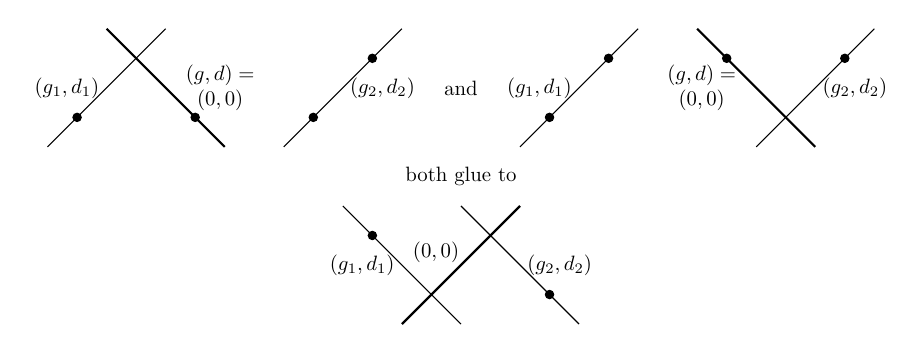
\begin{tikzpicture}[scale=.75,every node/.style={transform shape}]
  \draw (0,0) -- node[left]{$(g_1,d_1)$} (2,2);
  \draw[thick] (1,2) -- node[right]{\begin{tabular}{c} $(g,d)=$ \\ $(0,0)$ \end{tabular}} (3,0);
  \draw[fill=black] (.5,.5) circle[radius=2pt] (2.5,.5) circle[radius=2pt];
  \draw (4,0) -- node[right]{$(g_2,d_2)$}(6,2);
  \draw[fill=black] (4.5,.5) circle[radius=2pt] (5.5,1.5) circle[radius=2pt];
  
  \draw (7,1) node{and};
  
  \draw (8,0) -- node[left]{$(g_1,d_1)$} (10,2);
  \draw[fill=black] (8.5,.5) circle[radius=2pt] (9.5,1.5) circle[radius=2pt];
  \draw[thick] (11,2) -- node[left]{\begin{tabular}{c} $(g,d)=$ \\ $(0,0)$ \end{tabular}} (13,0);
  \draw (12,0) -- node[right]{$(g_2,d_2)$} (14,2);
  \draw[fill=black] (11.5,1.5) circle[radius=2pt] (13.5,1.5) circle[radius=2pt];

  \draw (7,-.5) node{both glue to};
  
  \draw (5,-1) -- node[left]{$(g_1,d_1)$}(7,-3) (7,-1) -- node[right]{$(g_2,d_2)$} (9,-3);
  \draw[thick] (6,-3) -- node[above left=-.1cm]{$(0,0)$} (8,-1);
  \draw[fill=black] (5.5,-1.5) circle[radius=2pt] (8.5,-2.5) circle[radius=2pt];
\end{tikzpicture}
\end{center}
Nevertheless $\psi$ has a natural perfect obstruction theory, given by $\LL_{\psi}$: we only need to show that it is supported in $[-1,0]$. Consider the exact triangle:
\begin{equation*} \psi^* \LL_{\MM_{g,n,\beta}^{\operatorname{wt}}} \to \LL_{\MM_{G,A,B}^{\operatorname{wt}}} \to \LL_\psi \xrightarrow{[1]} \end{equation*}
The first two terms are concentrated in degrees $[0,1]$, because they are the cotangent complexes of smooth Artin stacks. Therefore $\LL_\psi$ is concentrated in degrees $[-1,1]$. Furthermore, if we examine the long exact cohomology sequence near $\h^1(\LL_\psi)$ we find
\begin{equation*} \h^1(\psi^* \LL_{\MM_{g,n,\beta}^{\operatorname{wt}}}) \to \h^1(\LL_{\MM_{G,A,B}^{\operatorname{wt}}}) \to \h^1(\LL_\psi) \to 0 \end{equation*}
and hence we must show that the first map is surjective. But this is dual to the map which takes an infinitesimal automorphism of the disconnected curve to an infinitesimal automorphism of the corresponding connected curve (obtained by glueing together the ``nodal'' marked points). The space of infinitesimal automorphisms of a nodal curve splits into a direct sum of infinitesimal automorphisms of each component; since the glueing does not affect the components, we see that this map is an isomorphism. Hence $\h^1(\LL_\psi) = 0$ as claimed; morally this follows from the fact that the fibres of $\psi$ are Deligne--Mumford.

Hence there is a virtual pull-back map $\psi^!$ which defines a class
\begin{equation*}\psi^! \virt{\Q{g}{n}{X}{\beta}} \end{equation*}
on $\mathcal{D}^{\mathcal{Q}}(X,G,A,B)$. This is the same class as the one induced by the following perfect obstruction theory
\begin{equation*} \varphi^* \EE_{\rho_Q} \to \LL_{\rho_D} \end{equation*}
by functoriality of virtual pull-backs.

Finally if we look at \eqref{Product diagram} we see that $\ev_q^* \LL_{\Delta_{X^r}} \to \LL_h$ is a perfect obstruction theory for the map $h$. To summarise, we have a triangle
\begin{equation}\label{D-E-triangle}
 \begin{tikzcd}
  \D{X}{G,A}{B} \ar[dr,"\rho_D" below=0.1cm] \ar[rr,"h"] & & \E{X}{G,A}{B}\ar[dl,"\rho_E"] \\
& \MM_{G,A,B}^{\operatorname{wt}} &
 \end{tikzcd}
\end{equation}
where all three morphisms are equipped with perfect obstruction theories. We simply need to check that these fit together in a compatible triple.

\begin{lemma} \label{Lemma product class equals pullback class} There is a compatible triple
\begin{equation*}(h^* \EE_{\rho_E}, \varphi^*\EE_{\rho_Q}, \ev_q^*\LL_{\Delta_{X^r}}) \end{equation*}
for the triangle \eqref{D-E-triangle}. Hence by functoriality of virtual pull-backs we have:
\[
 \psi^!\virt{\Q{g}{n}{X}{\beta}}=\Delta_{X^r}^!\virt{\E{X}{G,A}{B}} = \virt{\D{X}{G,A}{B}}
\]
\end{lemma}
\begin{proof}
 We need to construct a morphism of triangles
 \bcd
 h^*\EE_{\rho_E}\ar[r]\ar[d] & \varphi^*\EE_{\rho_Q}\ar[r]\ar[d] & \ev_q^*\LL_{\Delta_{X^r}}\ar[r,"{[1]}"]\ar[d] & {} \\
 h^* \LL_{\rho_E}\ar[r] & \LL_{\rho_D}\ar[r] & \LL_h\ar[r,"{[1]}"] & {}
 \ecd
 
 Consider the following diagram:
\bcd
h^* \tilde{\mathcal{C}} \ar[r,"\nu"] \ar[rd,"\eta" below] & \varphi^* \mathcal{C} \ar[r] \ar[d] \ar[rd,phantom,"\square" right] & \mathcal{C} \ar[d,"\pi"] \\
& \D{X}{G,A}{B} \ar[r,"\varphi"] & \Q{g}{n}{X}{\beta}
\ecd
Here $\tilde{C}$ is the universal (disconnected) curve over $\E{X}{G,A}{B}$, which we have pulled back to $\D{X}{G,A}{B}$, while $\varphi^* \mathcal{C}$ is the universal curve over $\D{X}{G,A}{B}$. Therefore the map $\nu : h^* \tilde{\mathcal{C}} \to \varphi^* \mathcal{C}$ is (fiberwise) a partial normalisation map given by normalising the nodes which connect the ``trunk'' of the centipede to the ``legs.''

There are natural sheaves $\mathcal{F}$ and $\tilde{\mathcal{F}}$ on $\mathcal{C}$ and $h^* \tilde{\mathcal{C}}$ respectively, such that
\begin{align*} \varphi^*\EE_{\rho_Q}^\vee & = \R \pi_* \mathcal{F} \\
h^* \EE_{\rho_E}^\vee & = \R \eta_* \tilde{\mathcal{F}} \end{align*}
Furthermore $\nu^*\mathcal{F}\simeq\tilde{\mathcal{F}}$, hence by tensoring the partial normalisation short exact sequence
\begin{equation*} 0 \to \OO_{\varphi^*{\mathcal{C}}} \to \nu_* \OO_{h^* \tilde{\mathcal{C}}} \to \OO_q \to 0 \end{equation*}
with $\mathcal{F}$ and applying the projection formula, we obtain
\begin{equation*} 0 \to \mathcal{F} \to \nu_* \tilde{\mathcal{F}} \to \mathcal{F}_q \to 0 \end{equation*}
on $\varphi^*\mathcal{C}$, where $q$ is the locus of nodes connecting the trunk to the spine. (The fact that the morphism on the left is injective follows by applying the Snake Lemma to the short exact sequence defining $\mathcal{F}$.) To this we can apply $\R \pi_*$ to obtain an exact triangle
\begin{equation} \label{Normalisation exact triangle} \R \pi_* \mathcal{F} \to \R \eta_* \tilde{\mathcal{F}} \to \R \pi_* \mathcal{F}_q \xrightarrow{[1]} \end{equation}
Finally, notice that, since quasimaps are required not to have base-points at the nodes, the fibre of the sheaf $\mathcal F$ at each of the nodes $q$ can actually be identified with the tangent to the toric variety $X$ at the image of the node itself, i.e. $\R \pi_* \mathcal{F}_q \cong \ev_q^* \TT_{X^r}= \ev_q^* \mathbf{\operatorname{T}}_{\Delta_{X^r}}[-1]$. Dualising sequence \eqref{Normalisation exact triangle} we obtain
\begin{equation*} h^* \EE_{\rho_E} \to \varphi^* \EE_{\rho_Q} \to \ev_q^* \EE_{\Delta_{X^r}} \xrightarrow{[1]} \end{equation*}
as required. \end{proof}
\subsection{Comparison with the GIT construction} \label{Section comparison with GIT construction}

Let $X$ be a smooth projective toric variety and $Y \hookrightarrow X$ a smooth very ample hypersurface. The complete linear system $|\OO_X(Y)|$ gives an embedding $i : X \hookrightarrow \PP^N$ such that $Y$ is the intersection of $X$ with a certain hyperplane $H$ inside $\PP^N$. We can define the moduli space of quasimaps to $Y$ via the following cartesian diagram:
\bcd
\Q{g}{n}{Y}{\beta}\ar[d]\ar[r]\ar[rd,phantom,"\square"] & \Q{g}{n}{H}{d} \ar[d,] \\
\Q{g}{n}{X}{\beta}\ar[r,"k"] & \Q{g}{n}{\PP^N}{d}
\ecd
where $d=i_*\beta$. Thus defined, this moduli space is easy to describe. Let $s_Y$ denote the section of $\OO_X(Y)$ cutting out $Y$ inside $X$. Recall from \S \ref{Subsection relative stable quasimaps} that for any quasimap
\begin{equation*} ((C,x_1,\ldots,x_n),(L_\rho,u_\rho)_{\rho \in \Sigma_X(1)}, (\varphi_m)_{m \in M_X}) \in \Q{g}{n}{X}{\beta} \end{equation*}
we can construct a section $u_Y$ of a line bundle $L_Y$ on $C$, which plays the role of the pull-back of $s_Y$ to $C$. Then
\begin{equation*} \Q{g}{n}{Y}{\beta} \subseteq \Q{g}{n}{X}{\beta} \end{equation*}
consists of those quasimaps such that $u_Y \equiv 0$.

The cartesian diagram above can also be used to endow $\Q{g}{n}{Y}{\beta}$ with a virtual class via virtual (or diagonal) pull-back along $k$.

We wish to compare this definition with the GIT approach of \cite{CFKM}. We view $Y$ as the GIT quotient of the affine cone $C(Y)\subseteq \mathbb A^{\Sigma_X(1)}$ with respect to the ``diagonal'' action of $G:=\Hom_{\mathbb Z}(\Pic(X),\Gm)\cong\Gm^{\rho_X}\hookrightarrow \Gm^{\Sigma_X(1)}$ (here $C(Y)$ is invariant because it is cut out by a homogeneous equation). Objects of $\om{Q}^{\operatorname{GIT}}_{g,n}(Y,\beta)$ are diagrams of the form
\bcd
P \ar[d] \ar[r] & C(Y) \\ 
C & \,
\ecd
where $P$ is a principal $G$-bundle and the horizontal map is $G$-equivariant. Equivalently, this is the data of $P$ and a section of the associated $C(Y)$-bundle:
\bcd
P\times_{G} C(Y) \ar[d,"\rho" left] \\
C \ar[u,bend right,"u"right]
\ecd
The obstruction theory on this space is defined relative to the stack $\mathfrak{Bun}_{G}$ parametrising principal $G$-bundles on the universal curve:
\begin{equation*} \mathcal{C}_{\MM} \to \MM_{g,n} \end{equation*}
It is given by:
\begin{equation*} \EE_{\om{Q}/\mathfrak{Bun}_G}^\vee = \R \pi_* (u^*\LL_\rho) \end{equation*}
where
\begin{equation*} \pi \colon \mathcal C_{\mathfrak{Bun}}\to\mathfrak{Bun}_{G} \end{equation*}
is the universal curve.

Notice that $\mathfrak{Bun}_{G}\simeq\times^r_{\MM_{g,n}} \mathfrak{Pic}$ by taking the line bundles $\bigoplus_{i=1}^{\rho_X} L^{(i)}=P\times_{G}\mathbb A^{\rho_X}\to C$ associated to the $G$-torsor $P\to C$. Furthermore, the $G$-equivariant embedding in a smooth stack
\bcd
P\times_{G} C_Y \ar[r,hook]\ar[d,"\rho" left] & P\times_{G}\mathbb A^{\lvert\Sigma_X(1)\rvert}\simeq \bigoplus_{\rho\in\Sigma_X(1)} L_{\rho}\ar[dl]\\
C \ar[u,bend right,"u"right] &
\ecd
gives us $u^*T^\bullet_\rho\simeq[\bigoplus_{\rho\in\Sigma_X(1)} \mathcal L_{\rho}\to E_{g,n,\beta}^Y]$, where $E_{g,n,\beta}^Y$ is the line bundle associated to the universal ones $(\mathcal L_\rho)$ by the same rule that takes $(\mathcal O_X(D_\rho))$ to $\mathcal O_X(Y)$, and the arrow is induced by $P_Y$. This shows that both the modular interpretation and the obstruction theory coincide.


\section{Intersection-theoretic lemmas}\label{appendix:intersection}

In this appendix we explicitly define the \emph{diagonal pull-back} along a morphism whose target is unobstructed (used in \cite{Ga}) and verify that this agrees with the virtual pull-back of \cite{Manolache-Pull} when both are defined. We also check that it satisfies some expected compatibility properties.

Consider a morphism of DM stacks $f\colon Y\to X$ over a smooth base $\mathfrak M$, such that $X$ is smooth over $\mathfrak M$ and $Y$ carries a virtual class given by a perfect obstruction theory $\EE_{Y/\mathfrak M}$. Then, for every Cartesian diagram
 \bcd
 G\ar[r,"g"]\ar[d,"q"]\ar[rd,phantom,"\Box"] & F\ar[d,"p"] \\
 Y\ar[r,"f"] & X 
 \ecd
and every class $\alpha\in \Achow_*(F)$, we may define
\[
 f^!_{\Delta}(\alpha)=\Delta_X^!([Y]^\text{vir}\times\alpha)\in \Achow_*(G)
\]
which we call the \emph{diagonal (virtual) pull-back}. We first show that it coincides with the usual virtual pull-back along $f$ in the presence of a compatible perfect obstruction theory for $f$.

\begin{lemma}\label{lem:diagonal_virtual_coincide}
Assume that there exists a relative obstruction theory $\EE_f$ compatible with $\EE_{Y/\mathfrak M}$ and the standard (unobstructed) obstruction theory for $X$, i.e:
 \bcd
 f^* \LL_{X/\mathfrak M} \ar[r] \ar[d,"\operatorname{Id}"] & \EE_{Y/\mathfrak M} \ar[r] \ar[d] & \EE_f \ar[r,"{[1]}"] \ar[d] & \, \\
 f^* \LL_{X/\mathfrak M} \ar[r] & \LL_{Y/\mathfrak M} \ar[r] & \LL_f \ar[r,"{[1]}"] & \,
 \ecd
 Then for every Cartesian diagram and every class $\alpha\in \Achow_*(F)$ as above,
 \[
  f^!_{\operatorname{v}}(\alpha)=f^!_\Delta(\alpha).
 \]
\end{lemma}
\begin{proof}

Consider the following cartesian diagram:
\bcd
G \ar[r,"q \times g"] \ar[d,"g"] \ar[rd,phantom,"\square"] & Y\times_{\mathfrak M}F \ar[r,"\pr_1"] \ar[d,"f \times \Id"] \ar[rd,phantom,"\square"] & Y \ar[d,"f"] \\
F \ar[r,"p \times \Id"] \ar[d,"p"] \ar[rd,phantom,"\square"] & X\times_{\mathfrak M} F \ar[r,"\pr_1"] \ar[d,"\Id \times p"] & X \\
X \ar[r,"\Delta_X"] & X\times_{\mathfrak M}X &
\ecd
Then, by commutativity of virtual pull-backs, we have
\begin{align*} \Delta_X^!([Y]^\text{vir}\times\alpha) & = \Delta^!((f^!_{\operatorname{v}}[X])\times\alpha) \\
& = \Delta_X^!(f^!_{\operatorname{v}}([X]\times\alpha)) \\
& = f^!_{\operatorname{v}}(\Delta_X^!([X]\times\alpha)) \\
& = f^!_{\operatorname{v}}(\alpha)
\end{align*}
as required.
\end{proof}

Secondly, we show that the \emph{diagonal} virtual pull-back behaves similarly to an ordinary virtual pull-back (e.g. commutes with other virtual pull-backs) even in the absence of a compatible perfect obstruction theory.

\begin{lemma} The \emph{diagonal} virtual pull-back morphism as defined above commutes with ordinary Gysin maps and with virtual pull-backs. \end{lemma}
\begin{proof} First consider the case of ordinary Gysin maps. We must consider a cartesian diagram:
\bcd
Y^{\prime \prime} \ar[r] \ar[d] \ar[rd,phantom,"\square"] & X^{\prime \prime} \ar[r] \ar[d] \ar[rd,phantom,"\square"] & S \ar[d,"k"] \\
Y^\prime \ar[r] \ar[d] \ar[rd,phantom,"\square"] & X^\prime \ar[r] \ar[d] & T \\
Y \ar[r,"f"] & X
\ecd
with $k$ a regular embedding and $f\colon Y\to X$ as before. We need to show that for all $\alpha \in A_*(X^\prime)$:
\begin{equation*} k^! f_{\Delta}^!(\alpha) = f^!_{\Delta} k^!(\alpha) \end{equation*}
We form the cartesian diagram:
\bcd
Y^{\prime \prime} \ar[r] \ar[d] \ar[rd,phantom,"\square"] & Y\times X^{\prime \prime} \ar[r] \ar[d] \ar[rd,phantom,"\square"] & S \ar[d,"k"] \\
Y^\prime \ar[r] \ar[d] \ar[rd,phantom,"\square"] & Y\times X^\prime \ar[r] \ar[d] & T \\
X \ar[r,"\Delta_X"] & X\times X &
\ecd
And apply commutativity of usual Gysin morphisms. In the case where $k$ is not a regular embedding but rather is equipped with a relative perfect obstruction theory, the same argument works with $k^!$ replaced by $k_{\text{v}}^!$.
\end{proof}

\bibliographystyle{alpha}
\bibliography{relqm}

\end{document}